\chapter{Operation of the Large Scale OWF network}\label{5}
Connecting a large scale offshore wind farm network to the offshore converter stations has always been a challenge. In the chapter, the operation scheme of the 2 GW offshore network is detailed. Firstly, the initial conditions of the converters are depicted and then the stage-wise synchronization and operation of the network is explained. Later, dynamic analysis is performed for severe disturbances in the network such as sudden disconnection of one set of \gls{WG} and a three phase line to ground fault in the middle of the cable.

\section{Pre-set conditions of the converters}
In order to analyse the dynamic and steady state operation of the network, the controllers and set points need to be initialised before charging. They are set as following:

\begin{itemize}
    \item \gls{MMC}-1:
    \begin{itemize}
        \item \gls{AC} voltage control, V$_{ac,ref}$ = 1 p.u.
        \item Islanded mode operation
    \end{itemize}
\end{itemize}

\begin{itemize}
    \item \gls{MMC}-2:
    \begin{itemize}
        \item Active power control, $I_{d\_ref}$ = 0
        \item Non-islanded mode operation
        \item Id priority
    \end{itemize}
\end{itemize}

\section{Charging of MMCs and converter transformers}
The \gls{AC} side of \gls{MMC}s are to be connected for charging scenario. Since the \gls{DC} side is connected to battery sources, the charging of \gls{HVDC} cables is not considered for this study. As mentioned in the previous chapter, \gls{MMC}-1 works as grid forming (U/F control) and \gls{MMC}-2 works as grid following (active power control). Once the simulation is started, the voltage reference for the \gls{MMC} bus is provided by \gls{MMC}-1 and both the \gls{MMC}s are synchronized with 66 kV voltage on the \gls{AC} side. The offshore converter transformers are also energized in this process. The synchronism between both the \gls{MMC}s can be viewed from the \gls{MMC} bus voltage in Figure \ref{fig:VACP_MMC_1_2_sync}. 1 p.u. is achieved when synchronized. There are no currents flowing through the \gls{MMC}s as the \gls{WG}s are not yet connected as shown in Figure \ref{fig:IABC_MMC_1_2_sync}.

\begin{figure}[H]
\centering
%\hspace*{-1.2cm}
    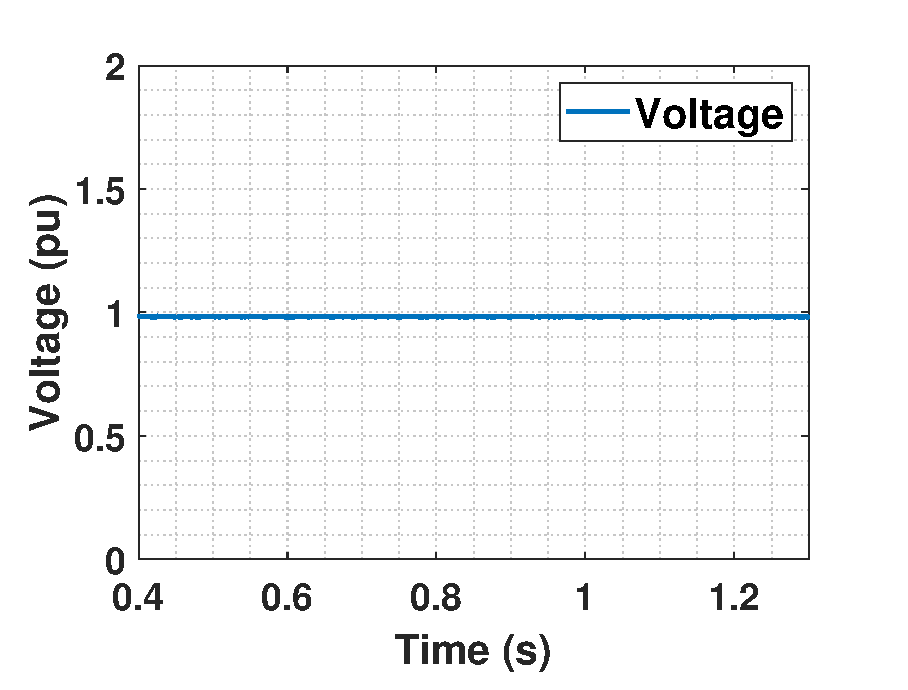
\includegraphics[height = 5.5cm,width = 8cm]{Diagrams/Chapter_5/VACP_MMC_1_2_sync.eps}
    \caption{Voltage at MMC common bus after synchronization}
    \label{fig:VACP_MMC_1_2_sync}
\end{figure}

\begin{figure}[H]
%\centering
\hspace*{-1.2cm}
    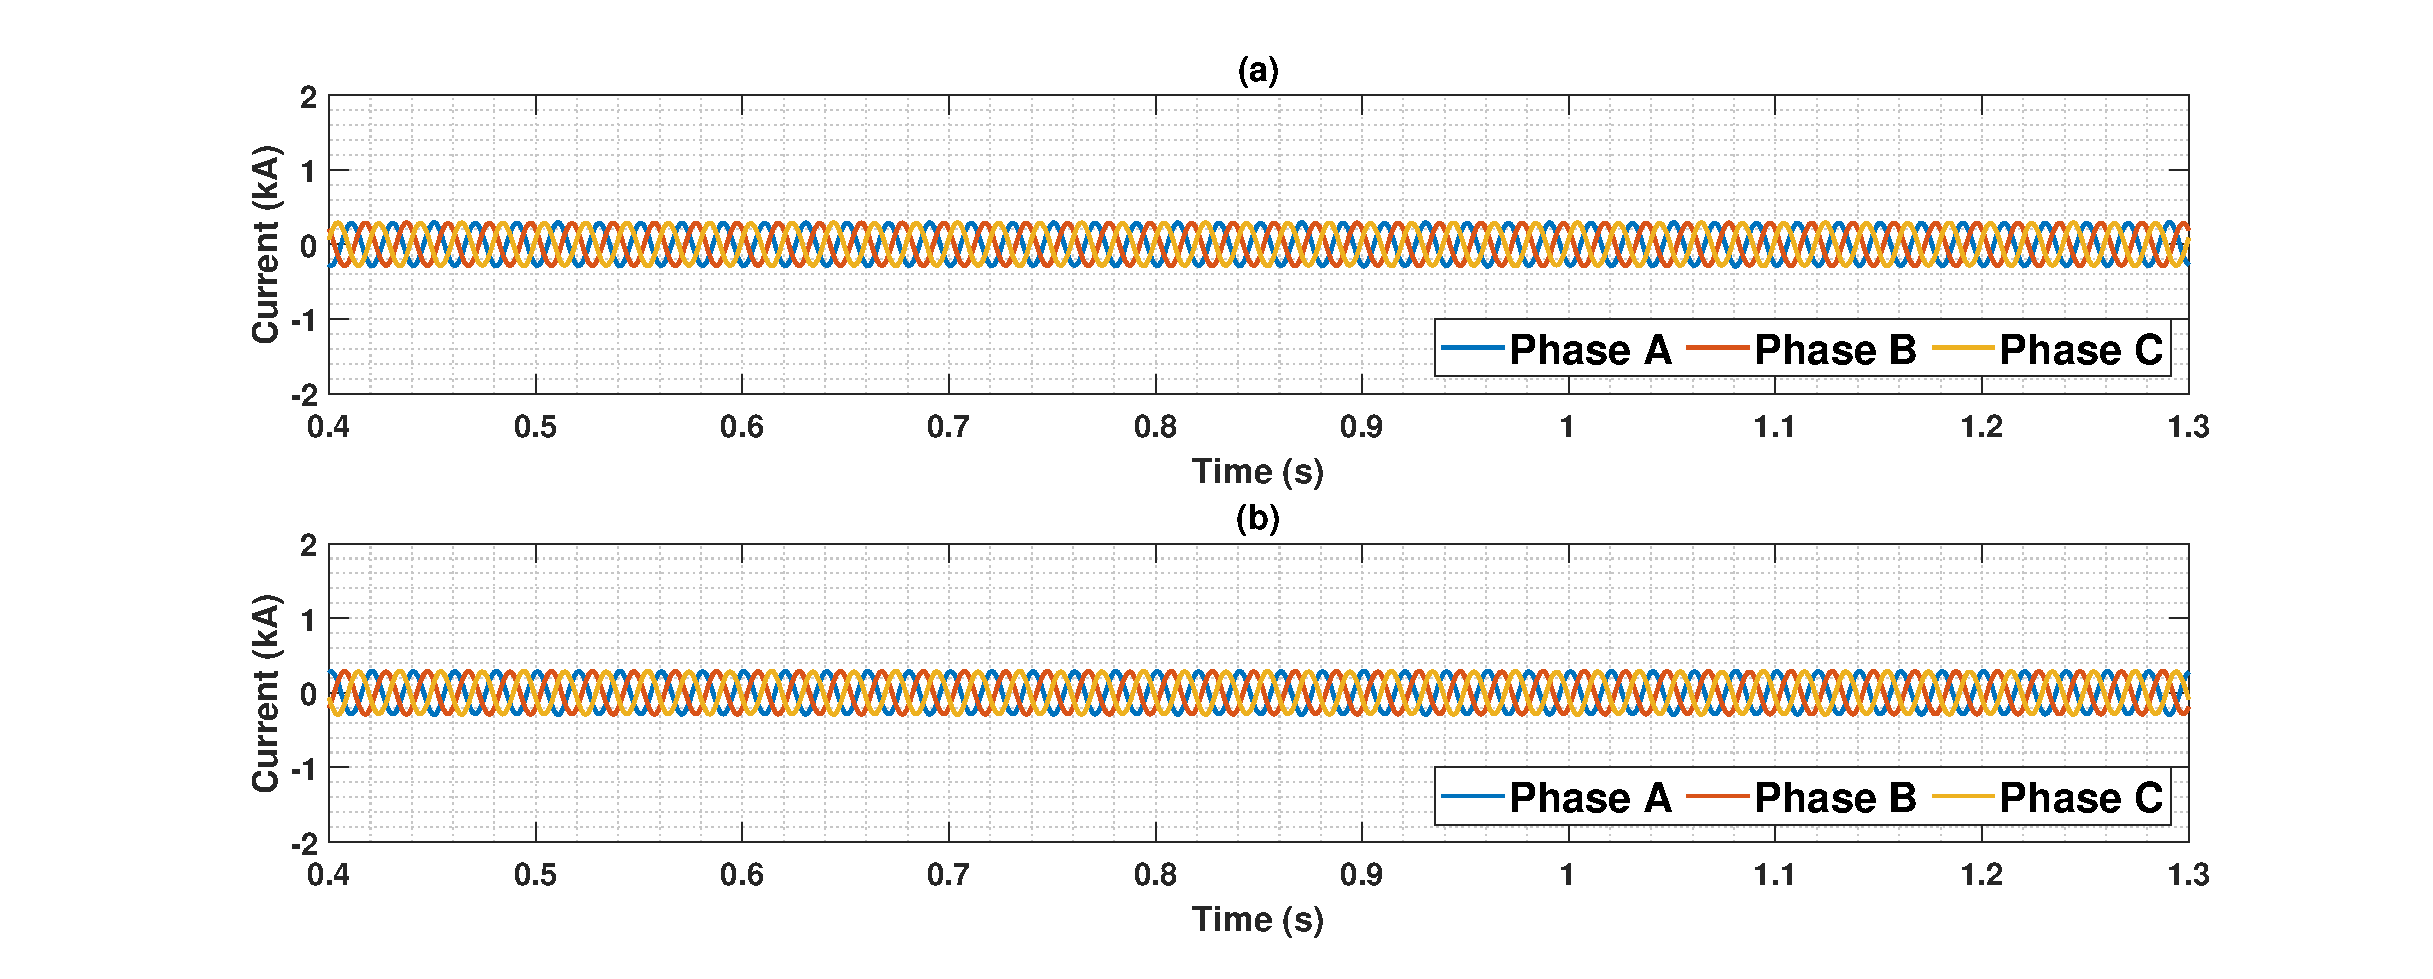
\includegraphics[height = 8.5cm,width = 18.5cm]{Diagrams/Chapter_5/IABC_MMC_1_2_sync.eps}
    \caption{Currents in a) MMC-1 bus and b) MMC-2 bus after synchronization}
    \label{fig:IABC_MMC_1_2_sync}
\end{figure}

\section{Energization of the HVAC cables and WGs}
The energization procedure of the \gls{AC} network followed in this work involves charging each \gls{HVAC} cable and the following \gls{WG}. In real scenario, such a procedure allows for operation of the \gls{WG}s that are tested and ready for commissioning even if other sets of \gls{WG}s are under construction. Initially cable-1 is charged and then \gls{WG}-1 is connected. The same is followed for the other sets of \gls{WG}s as well. Each \gls{WG} is rated at 6 MW nominal power capacity and they have a maximum scaling rated capacity of 500 MW. For the energization process, the \gls{WG}s are connected initially with lower generation of nearly 50 MW power to avoid surge of voltage at \gls{PCC} and to maintain the voltage within limits. Once stability is attained after connecting all the \gls{WG}s, the generation is incremented. Since power only flows through \gls{MMC}-1 until then, the increment can be until the maximum capacity of \gls{MMC}-1 i.e. 1 GW. All events are timed to take place at 0.5 seconds of the simulation.   

The cable-1 gets energized when the CB-1a circuit breaker, as shown in Figure \ref{fig:WT4_MMC2}, is switched on. The current in the cable is shown in Figure \ref{IABC_MMC_1_Cab1_Cab1charg}(b). The active power reference for the \gls{MMC}-2 is not changed and hence there is no power flowing through \gls{MMC}-2 bus and power flows only through \gls{MMC}-1 as seen from the currents of \gls{MMC}-1 in Figure \ref{IABC_MMC_1_Cab1_Cab1charg}(a). The slight disturbances observed during the switching operation, before the currents stabilize to a particular value, is due to the interaction between the controllers of \gls{MMC}-1 and \gls{MMC}-2. Voltage at the \gls{MMC} common bus is also increased slightly and set to a value of nearly 1.05 p.u. as seen in Figure \ref{VACP_MMC_bus_Cab1charg}.

\begin{figure}[H]
\centering
%\hspace*{-1.2cm}
    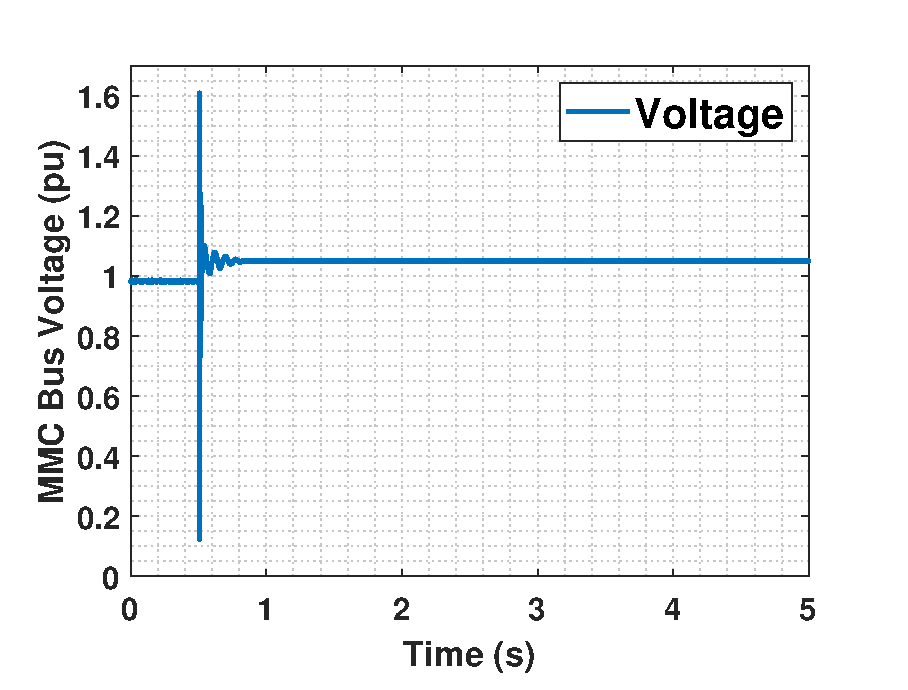
\includegraphics[height = 6.5cm,width = 9cm]{Diagrams/Chapter_5/VACP_MMC_bus_Cab1charg.eps}
    \caption{Voltage at MMC common bus after charging of cable-1}
    \label{VACP_MMC_bus_Cab1charg}
\end{figure}

\begin{figure}[H]
\centering
%\hspace*{-1.2cm}
    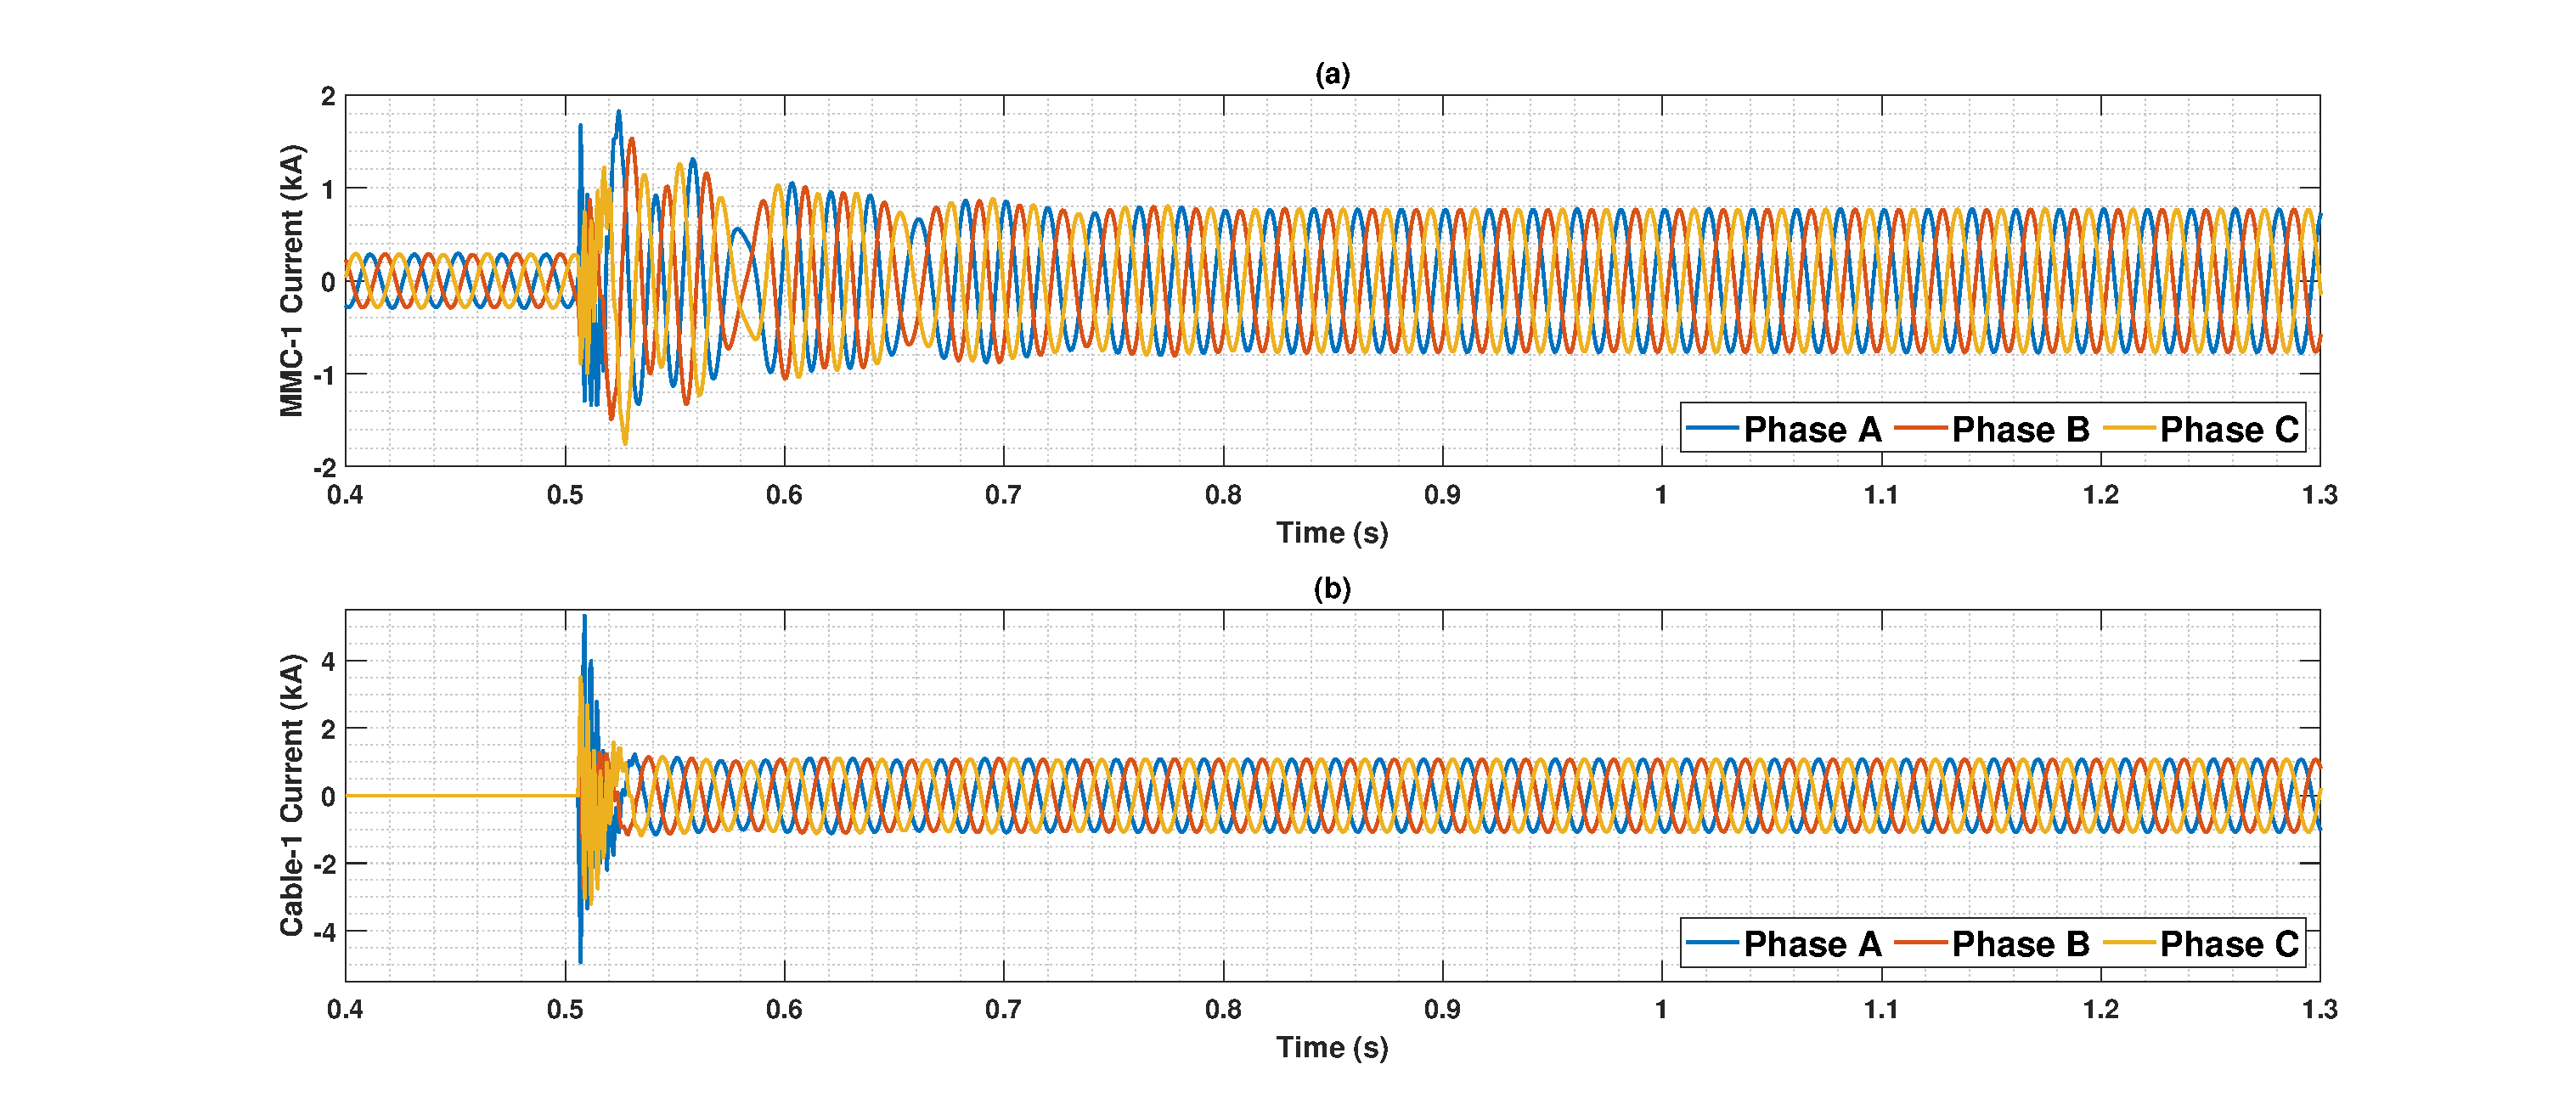
\includegraphics[height = 8.5cm,width = 16.5cm]{Diagrams/Chapter_5/IABC_MMC_1_Cab1_Cab1charg.eps}
    \caption{Charging of cable 1: a) Currents in MMC-1 b) Currents in cable-1}
    \label{IABC_MMC_1_Cab1_Cab1charg}
\end{figure}

After cable-1 has been charged, the breaker at the \gls{WG}-1 end (CB-1b) is switched on. \gls{WG}-1 gets connected to the network. As mentioned earlier, the \gls{WG}-1 is connected initially with less generation to keep the voltage at \gls{PCC}-1 within limits. The initial high voltage at the \gls{PCC}-1 before closing the breaker as seen in Figure \ref{VACP_WT1_WT1connect} is due to the capacitance in the DC link. Once the breaker is closed, the voltage is maintained at nearly 1 pu as shown in Figure \ref{VACP_WT1_WT1connect} and currents in the \gls{PCC}-1 also increase as shown in Figure \ref{IABC_WT1_WT1connect}. The \gls{WG} starts generating 50 MW and this flows through \gls{MMC}-1 as shown in Figure \ref{P_MMC_1_2_WT1234connect} a). In a similar way all the other \gls{WG}s are connected. All \gls{WG}s are connected with 50 MW generation and a total power of 200 MW through \gls{MMC}-1 after connection of \gls{WG}-1, \gls{WG}-2, \gls{WG}-3 and \gls{WG}-4 can be seen from the graphs in Figure \ref{P_MMC_1_2_WT1234connect} a), b), c) and d) respectively. There is no flow of active power in \gls{MMC}-2 since the rated capacity of \gls{MMC}-1 is yet to be reached.

\begin{figure}[H]
\centering
%\hspace*{-1.2cm}
    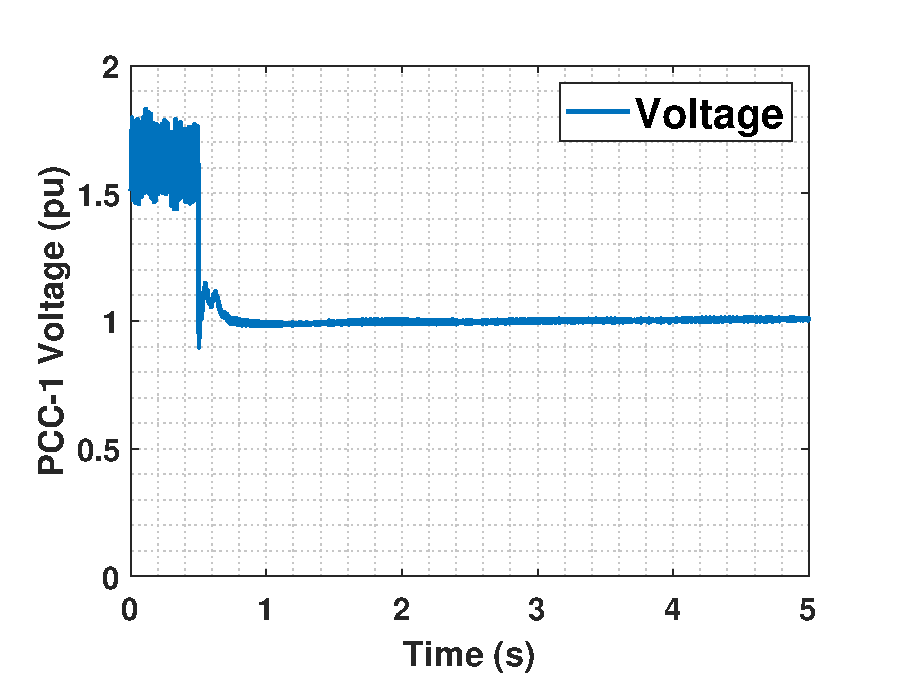
\includegraphics[height = 5.5cm,width = 8cm]{Diagrams/Chapter_5/VACP_WT1_WT1connect.eps}
    \caption{Voltage at PCC-1 after connecting WG-1 to the network}
    \label{VACP_WT1_WT1connect}
\end{figure}

\begin{figure}[H]
\centering
%\hspace*{-1.2cm}
    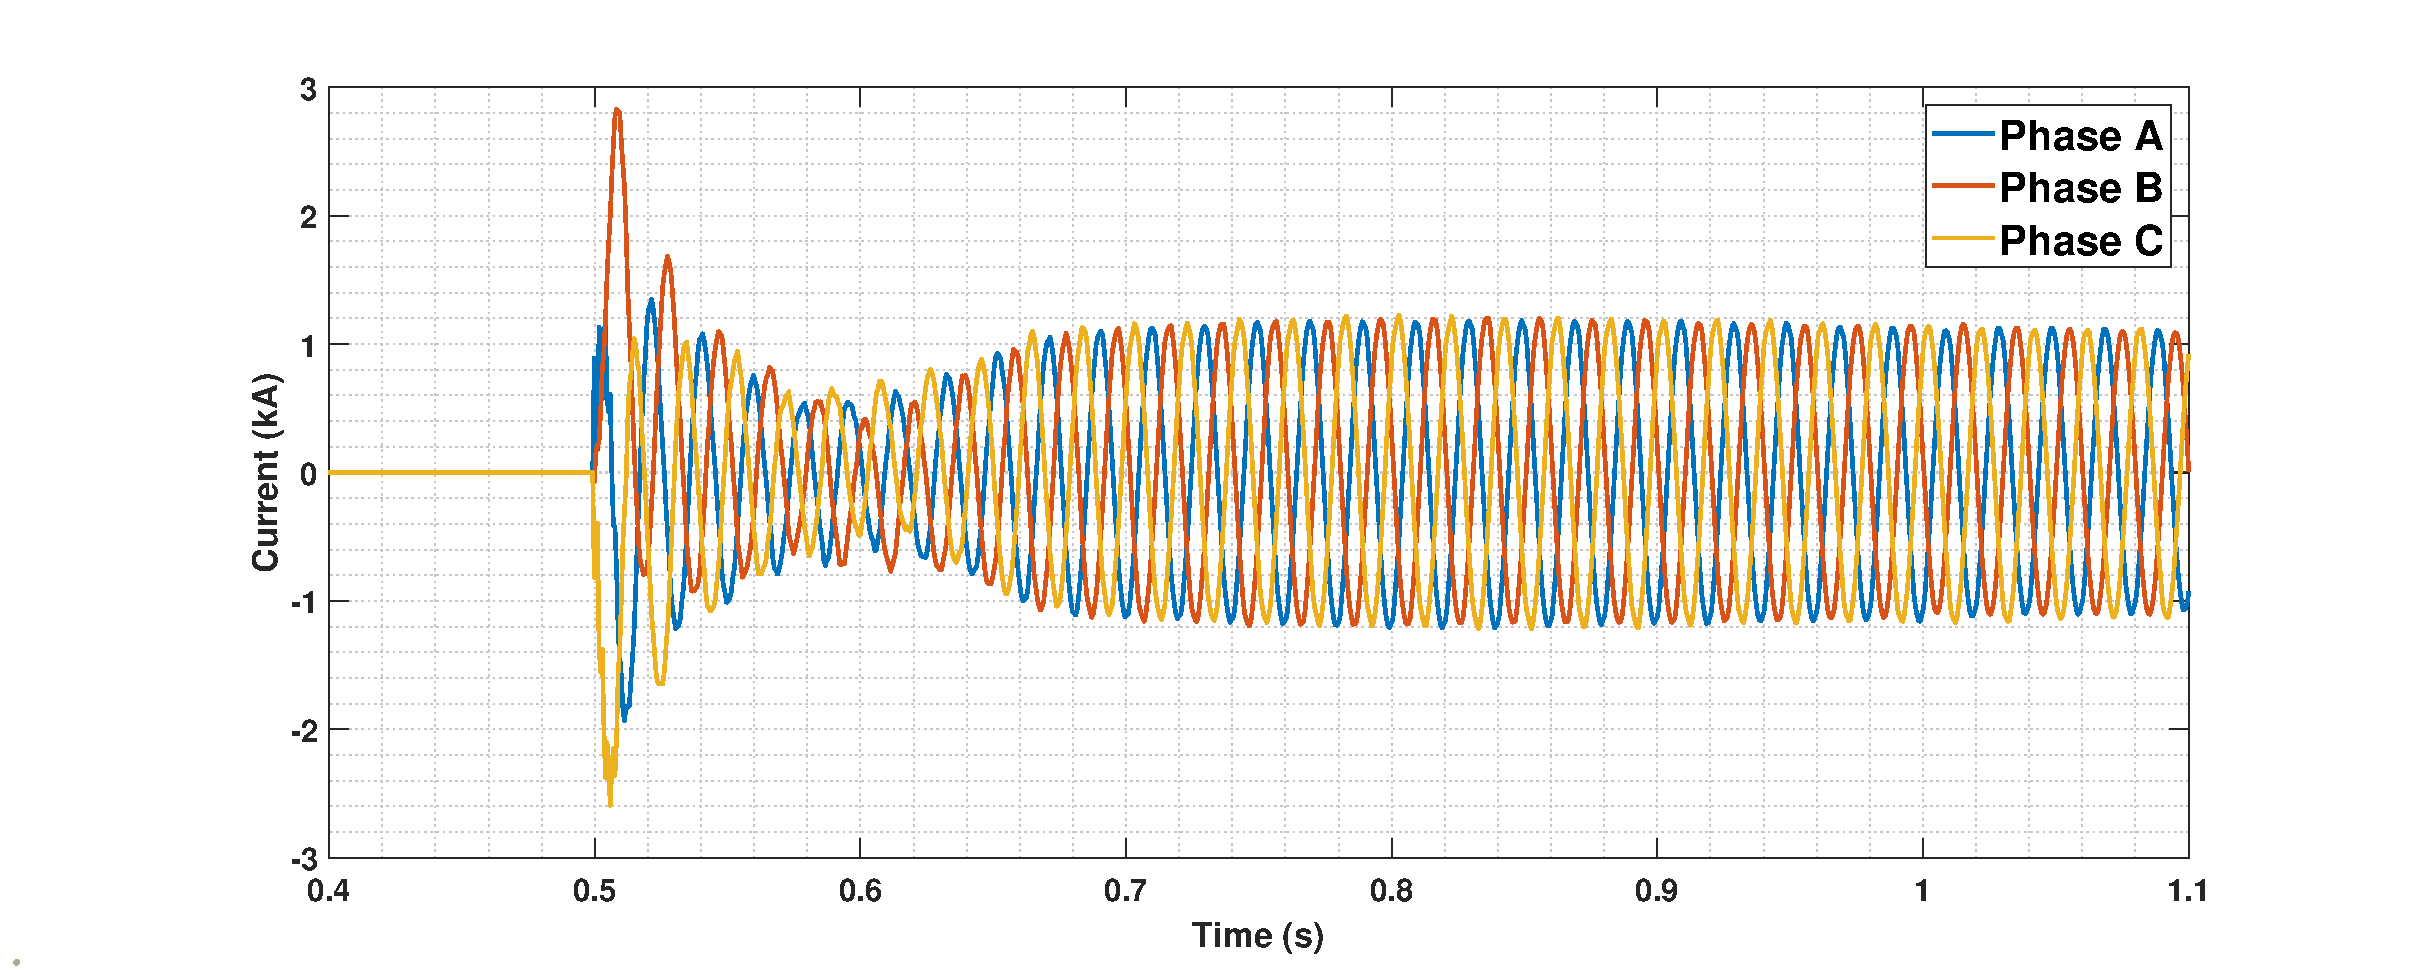
\includegraphics[height = 6cm,width = 16.5cm]{Diagrams/Chapter_5/IABC_WT1_WT1connect.eps}
    \caption{Currents at PCC-1 upon connecting WG-1 to the network}
    \label{IABC_WT1_WT1connect}
\end{figure}

\begin{figure}[H]
%\centering
\hspace*{-1.2cm}
    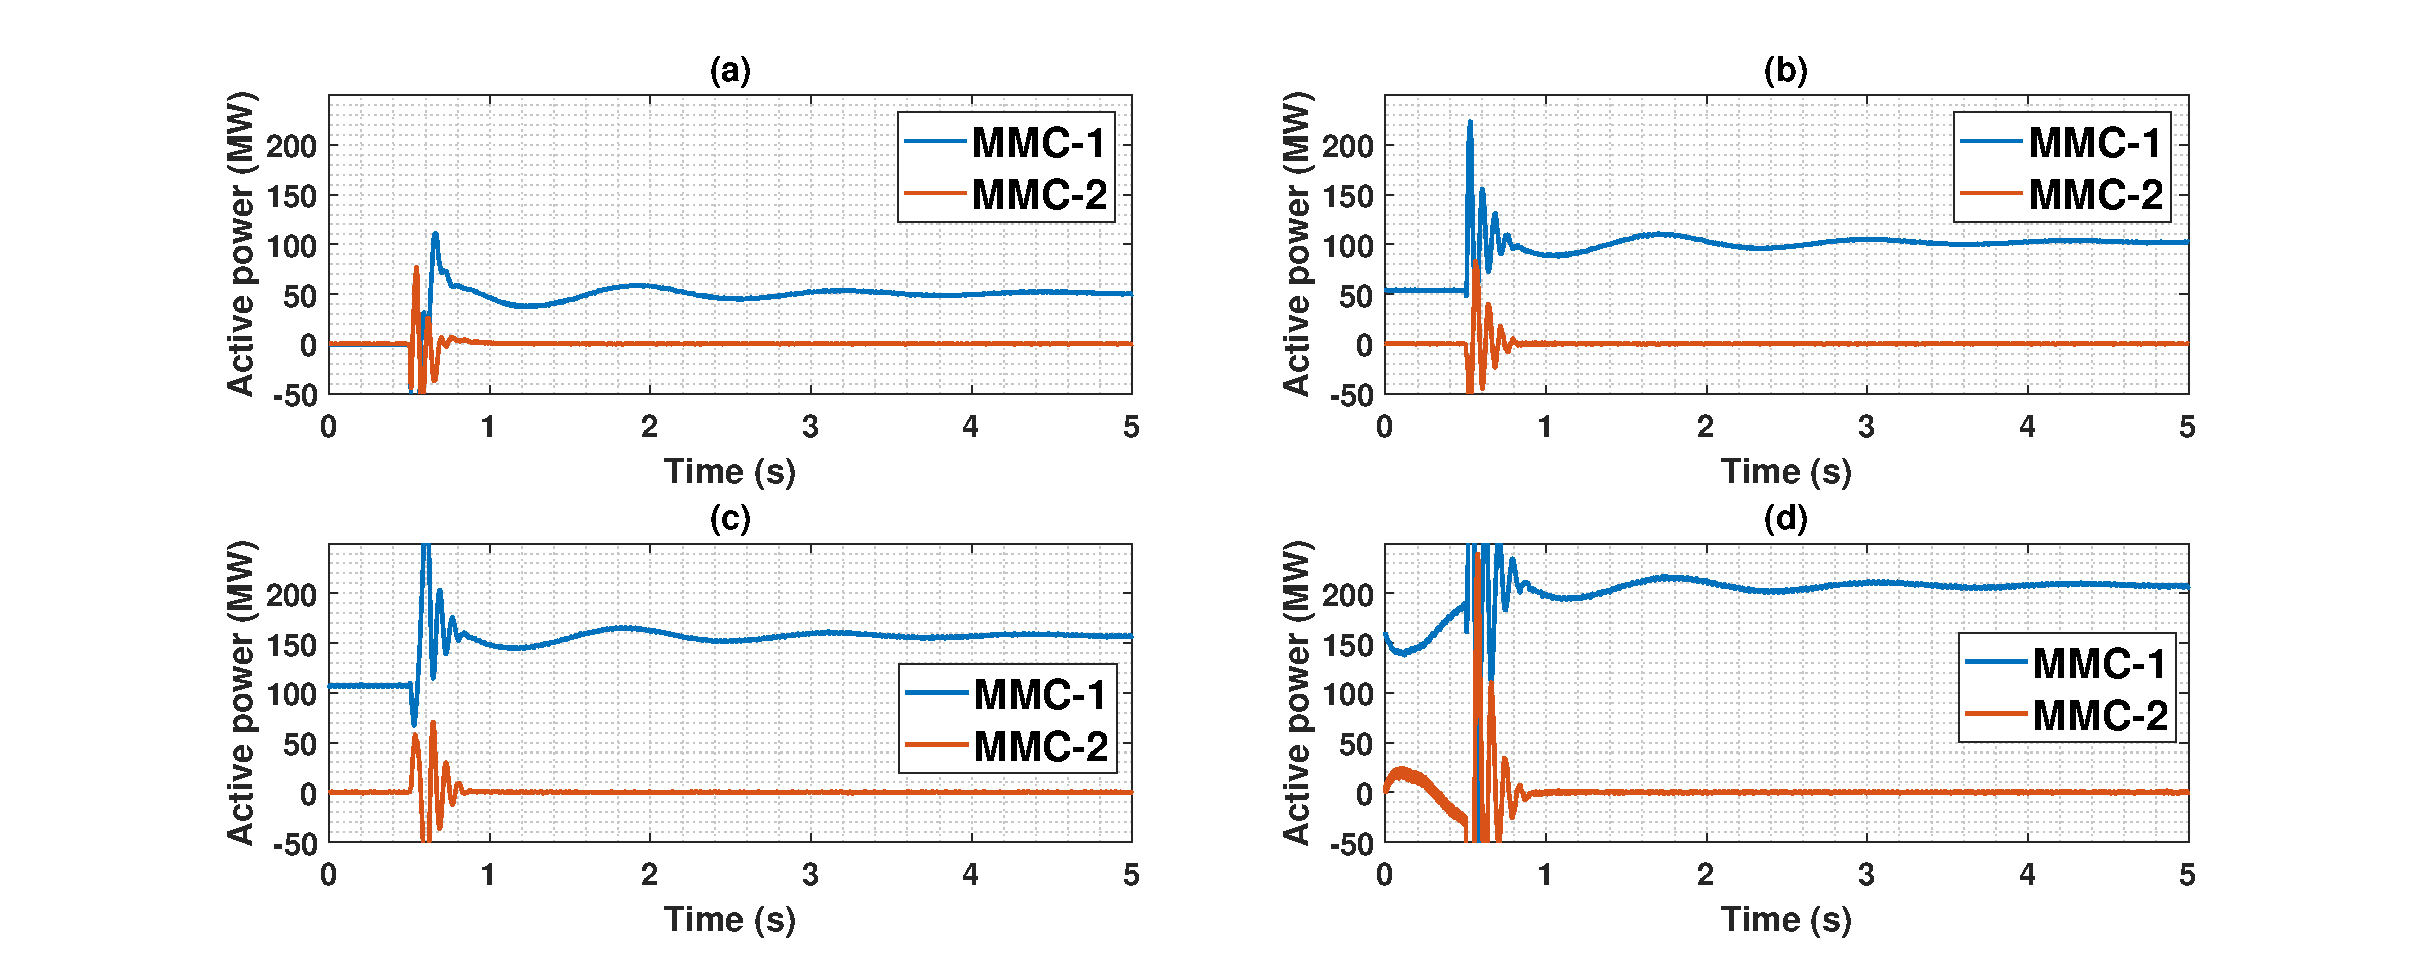
\includegraphics[height = 8.5cm,width = 18.5cm]{Diagrams/Chapter_5/P_MMC_1_2_WT1234connect.eps}
    \caption{Active power in \gls{MMC}-1 and \gls{MMC}-2 upon connecting a) WG-1, b) WG-2, c) WG-3 and d) WG-4}
    \label{P_MMC_1_2_WT1234connect}
\end{figure}

Once the system gets stabilized, the generation is increased and voltage is ensured to be within limits at all \gls{PCC}s. The power flow to the \gls{MMC}-2 is to be controlled in the next step. This is done by controlling the active power reference of \gls{MMC}-2. It is changed in such a manner that there is equal distribution of power between \gls{MMC}-1 and \gls{MMC}-2. For this study, it is modelled such that all \gls{WG}s have the same scaling of power and hence they all produce the same amount of power at every instant. In small steps, the generation of the \gls{WG}s are increased and correspondingly the reference power to \gls{MMC}-2 is also changed. Finally, the \gls{WG}s are made to generate 500 MW each and the total of nearly 2 GW power is equally split between \gls{MMC}-1 and \gls{MMC}-2 as shown in Figure \ref{P_MMC_1_2_WT1234connect}.

\begin{figure}[H]
\centering
%\hspace*{-1.2cm}
    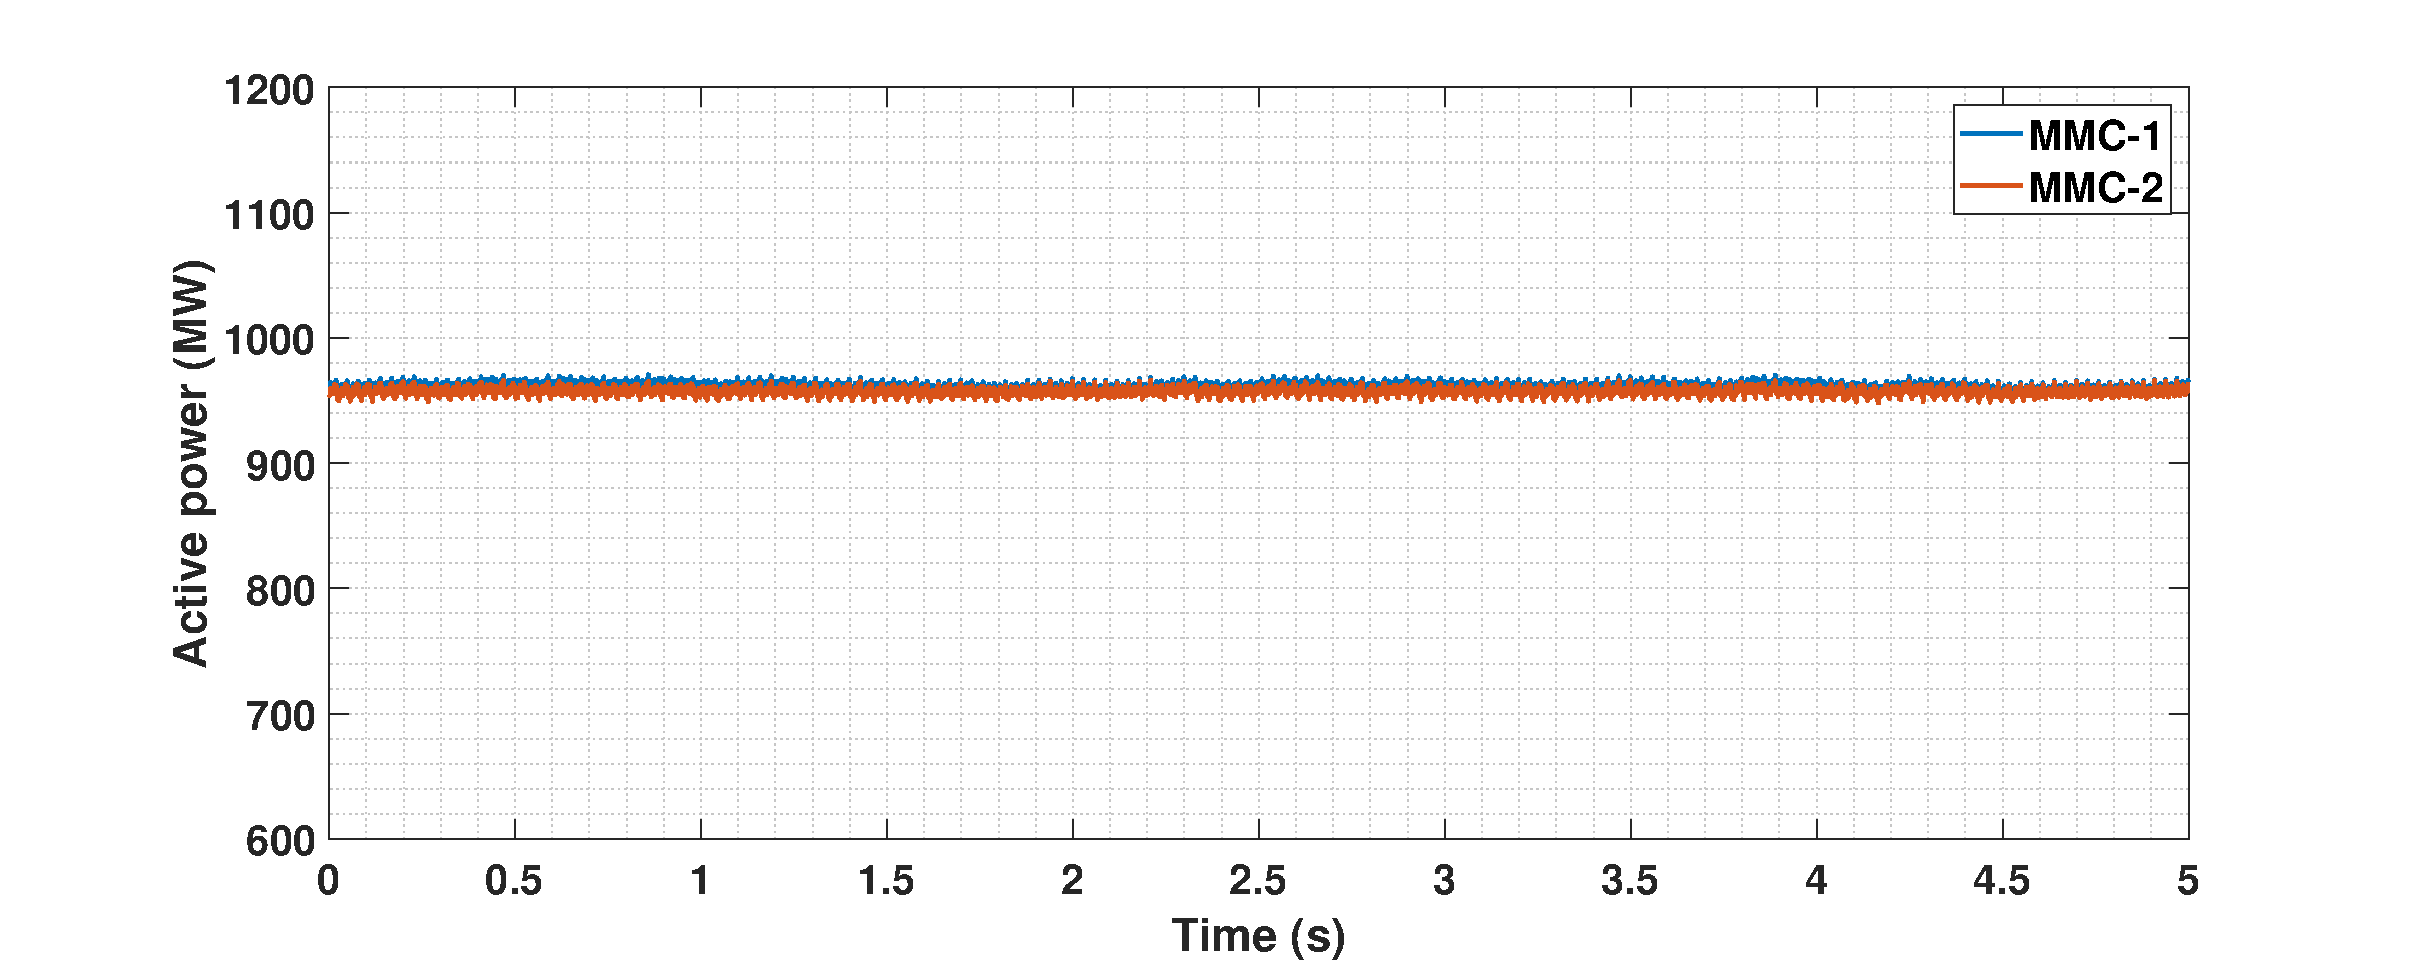
\includegraphics[height = 5.5cm,width = 8cm]{Diagrams/Chapter_5/P_MMC_1_2_All_WTconnect.eps}
    \caption{Active power in MMC-1 and MMC-2 upon connecting all 4 WGs in full generation}
    \label{P_MMC_1_2_All_WTconnect}
\end{figure}

The synchronization of both \gls{MMC}s and the energization of the offshore \gls{AC} grid is done successfully. The offshore \gls{AC} grid converters and cables now operate at a voltage of 66 kV, the \gls{HVDC} voltage is set to 640 kV and the total active power transmitted is nearly 2 GW in the network. Frequency of the system is stabilized at 50 Hz and the power system is said to be operating in the steady state condition.  

\section{Dynamic performance analysis}
Fault events and perturbations occur in the grid and the components in the system must be able to withstand the voltage surges and fault currents for a specific time span. To analyse the performance and coordination of the different controllers in the network, the system was tested for different cases of perturbations.  

\subsection{Disconnection of one set of WG}
The first event is a sudden disconnection of 1 set of \gls{WG}. \gls{WG}-2 is permanently disconnected from the circuit by opening the breaker connected towards \gls{WG}-2 cable end (CB-2a) at 500 ms. Once the breaker is open, the generation is lost and the current flowing reduces as witnessed in Figure \ref{IABC_MMC_1_2_WT2off}. The power flow is reduced through \gls{MMC}-1 as shown in Figure \ref{P_MMC_1_2_WT2off} due to the fact that \gls{MMC}-1 is the one in grid forming control (absorbs and provides power) and also the active power reference of \gls{MMC}-2 is unchanged.
In the post fault period, since the active power reference of \gls{MMC}-2 is not changed and the total amount of power is reduced, the flow of power is slightly more in \gls{MMC}-2 than in its pre-fault state as can be seen in Figure \ref{P_MMC_1_2_WT2off}. The \gls{MMC}-2 is seen to be operating with the maximum rated capacity of 1 GW in this condition.

\begin{figure}[H]
\centering
%\hspace*{-1.2cm}
    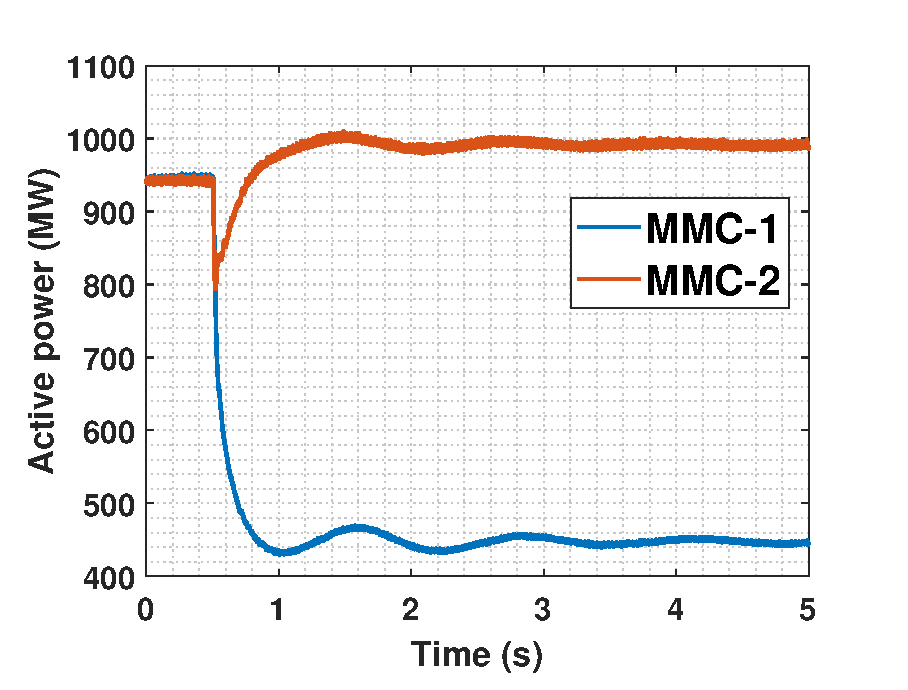
\includegraphics[height = 5.5cm,width = 8cm]{Diagrams/Chapter_5/P_MMC_1_2_WT2off.eps}
    \caption{Active power in MMC-1 connected bus and MMC-2 connected bus during WG-2 disconnection event}
    \label{P_MMC_1_2_WT2off}
\end{figure}

\begin{figure}[H]
%\centering
\hspace*{-1.2cm}
    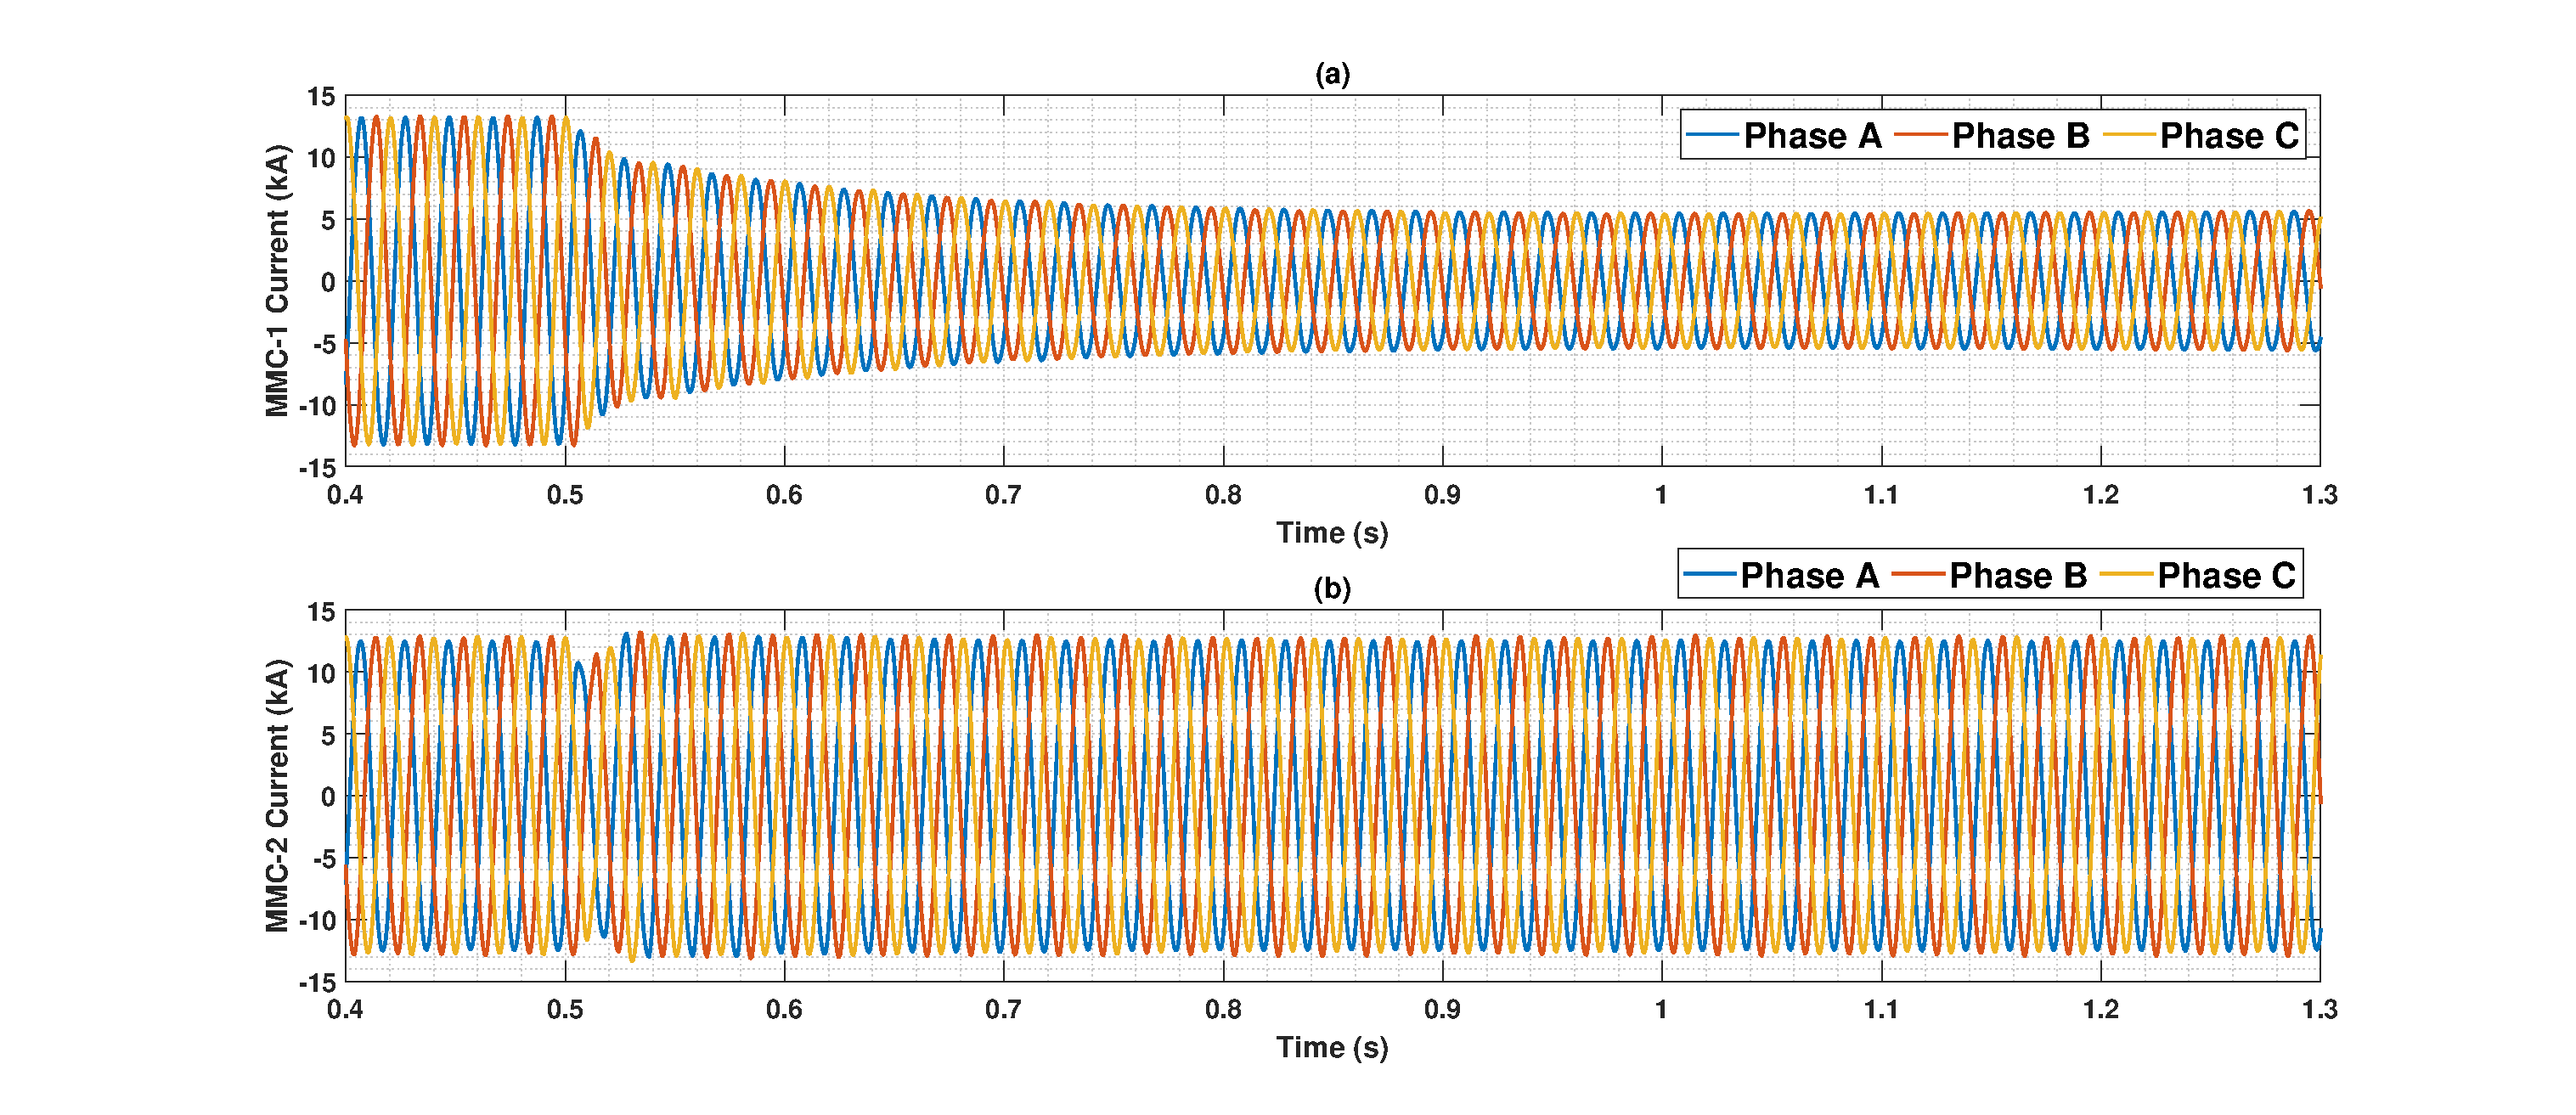
\includegraphics[height =8.5cm,width = 18.5cm]{Diagrams/Chapter_5/IABC_MMC_1_2_WT2off.eps}
    \caption{Currents in a) MMC-1 bus and b) MMC-2 bus during WG-2 disconnection event}
    \label{IABC_MMC_1_2_WT2off}
\end{figure}


In the \gls{OWF} side, the voltage at \gls{PCC}-2 goes to instability and is in the condition as before energizing. The currents and the voltages at the \gls{PCC}s of \gls{WG}s 1,3 and 4 observe transient during the instant of fault and then comes to a stable state. The voltage drops and there is a rise in current during the instant of fault, as shown in Figure \ref{IABC_WT1234_WT2off} and Figure \ref{VACP_WT134_WT2off} respectively. The voltage in the post-fault is slightly higher than pre-fault state. This happens in order to maintain sufficient amount of power to be transmitted to \gls{MMC}-2 for the specified active power reference without \gls{WG}-2 in the network. These can be observed in the graphs in Figure \ref{VACP_WT134_WT2off} and Figure \ref{IABC_WT1234_WT2off}.

\begin{figure}[H]
\centering
%\hspace*{-1.2cm}
    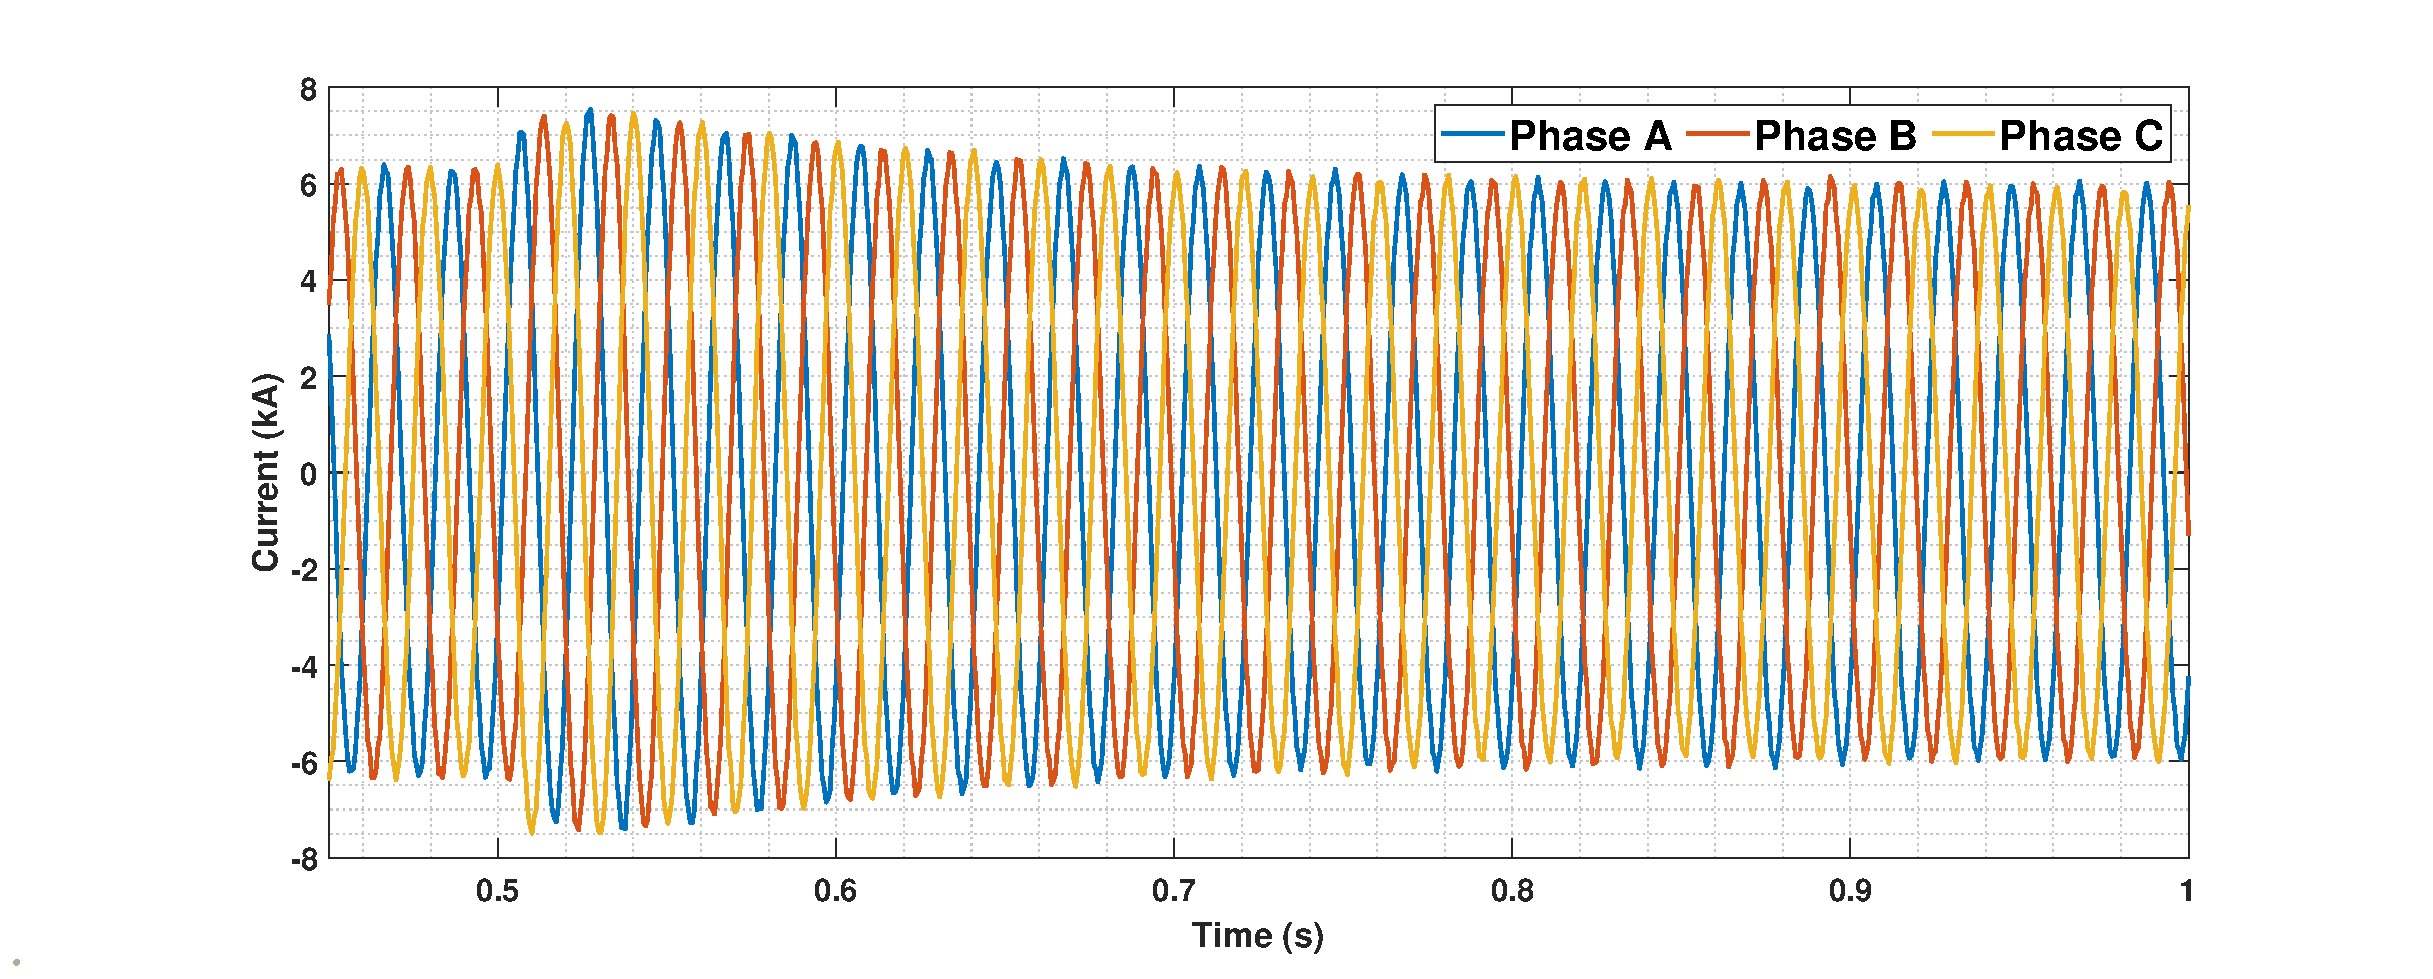
\includegraphics[height = 6.5cm,width = 17.5cm]{Diagrams/Chapter_5/IABC_WT1234_WT2off.eps}
    \caption{Currents at PCC-1, 3 and 4 during WG-2 disconnection event}
    \label{IABC_WT1234_WT2off}
\end{figure}

\begin{figure}[H]
\centering
%\hspace*{-1.2cm}
    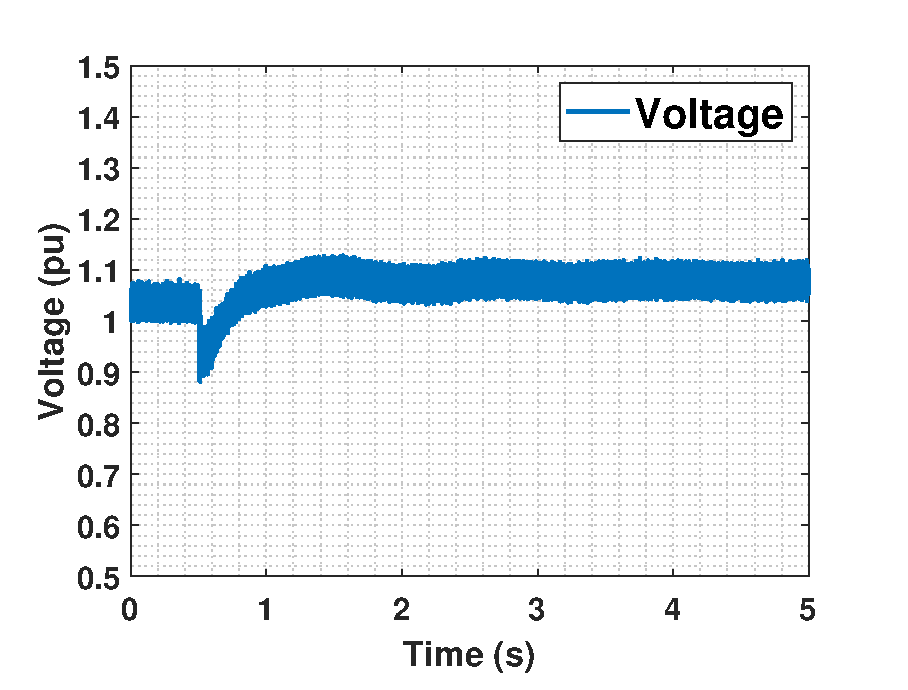
\includegraphics[height = 7.5cm,width = 9cm]{Diagrams/Chapter_5/VACP_WT134_WT2off.eps}
    \caption{Voltages at PCC-1, 3 and 4 during WG-2 disconnection event}
    \label{VACP_WT134_WT2off}
\end{figure}

\subsection{Three phase line to ground fault}

Before the application of three-phase line to ground fault, a logic to operate the circuit breaker (CB-1a) at the cable-1 end is developed as shown in Figure \ref{fig:Fault_logic}. For the fault, the line to ground fault logic available in RSCAD library is used.

\subsubsection{Circuit breaker operation}\label{Fault logic and cb}
Once the system is fully operational after connecting all the four \gls{WG}s and achieving 1 GW power in each \gls{MMC}s, the 'Activ' switch in Figure \ref{fig:Fault_logic} is turned on. This is done to provide the switching operation of the breaker. The system is still in steady state condition. This loop allows comparison of the RMS current ($I_{rms}$) and the maximum phase current ($I_{phase\_max}$) and provides control action for the circuit breaker. Once fault is applied, when $I_{rms}$ becomes greater than $I_{phase\_max}$, the SR flip flop detects the change and holds a value of zero for the signal 'SWD2A' (\gls{CB} operating signal). This action causes the breaker to open. The delay block before the signal provides the time delay for the operation of \gls{CB} after the fault has been detected.

\begin{figure}[H]
\centering
%\hspace*{-1.2cm}
    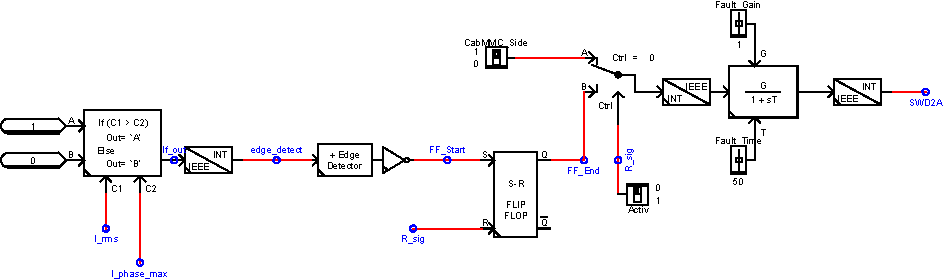
\includegraphics[height = 4.5cm,width = 14.5cm]{Diagrams/Chapter_5/Fault_logic_New.pdf}
    \caption{Circuit breaker operation logic}
    \label{fig:Fault_logic}
\end{figure}

In order to analyse the stability of the system under dynamic conditions, a permanent three-phase line to ground fault is applied in the middle of the \gls{WG}-1 cable. This allows the user to analyse the performance of the various control structures present in the network. The response of the system is recorded and depicted in Figure \ref{1516_3phaseSC} to Figure \ref{18_3phaseSC} for the event. The logic developed detects the over current in CB-1a at the cable-1 end which results in opening of the breaker. The overcurrent is detected at 0.53 seconds of the simulation from the developed logic and a short delay of nearly 12 ms is provided to open the breaker after the fault has been detected similar to a practical scenario (Figure \ref{Circuit_breaker_3phasefault}). After the breaker has been opened, the \gls{WG}-1 is taken out from the network and the total power provided to the onshore network is reduced. The total power in the pre-fault period is 2 GW and after the fault the total power is reduced to 1500 MW. This can be observed from the graphs in Figure \ref{17_3phaseSC}. As in the previous case, the power flow is reduced through \gls{MMC}-1 as shown in Figure \ref{1516_3phaseSC}. The graphs also depict that, after the breaker has been opened, the system gets to a stable operation. 

\begin{figure}[H]
\centering
%\hspace*{-1.2cm}
    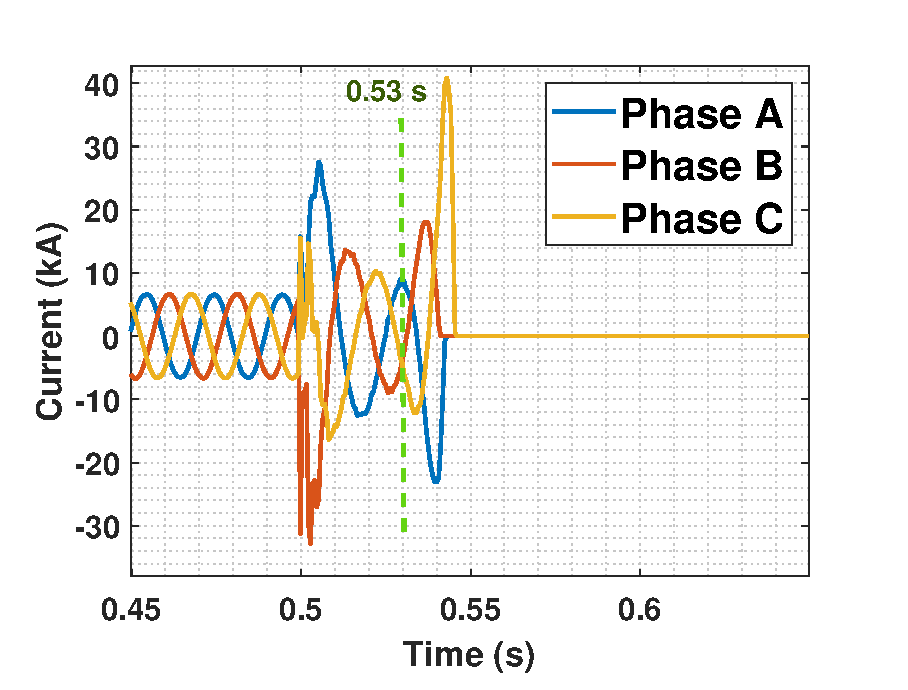
\includegraphics[height = 6.5cm,width = 9.5cm]{Diagrams/Chapter_5/IABC_CB_3phaseSC_new_2.eps}
    \caption{Currents in circuit breaker (CB-1a) during three-phase line to ground fault in cable-1}
    \label{Circuit_breaker_3phasefault}
\end{figure}

A major observation can be viewed from the profile of transients during the fault in the currents of both the \gls{MMC}s. The initial transients is due to the occurrence of fault until it is detected at 0.53 s. The transients in currents after the breaker has been opened (at 0.59 s) are complementary in both \gls{MMC}s. It means that \gls{MMC}-1 has the dominating control during steady-state conditions and after the breaker has been operated. 

\begin{figure}[H]
%\centering
\hspace*{-1.2cm}
    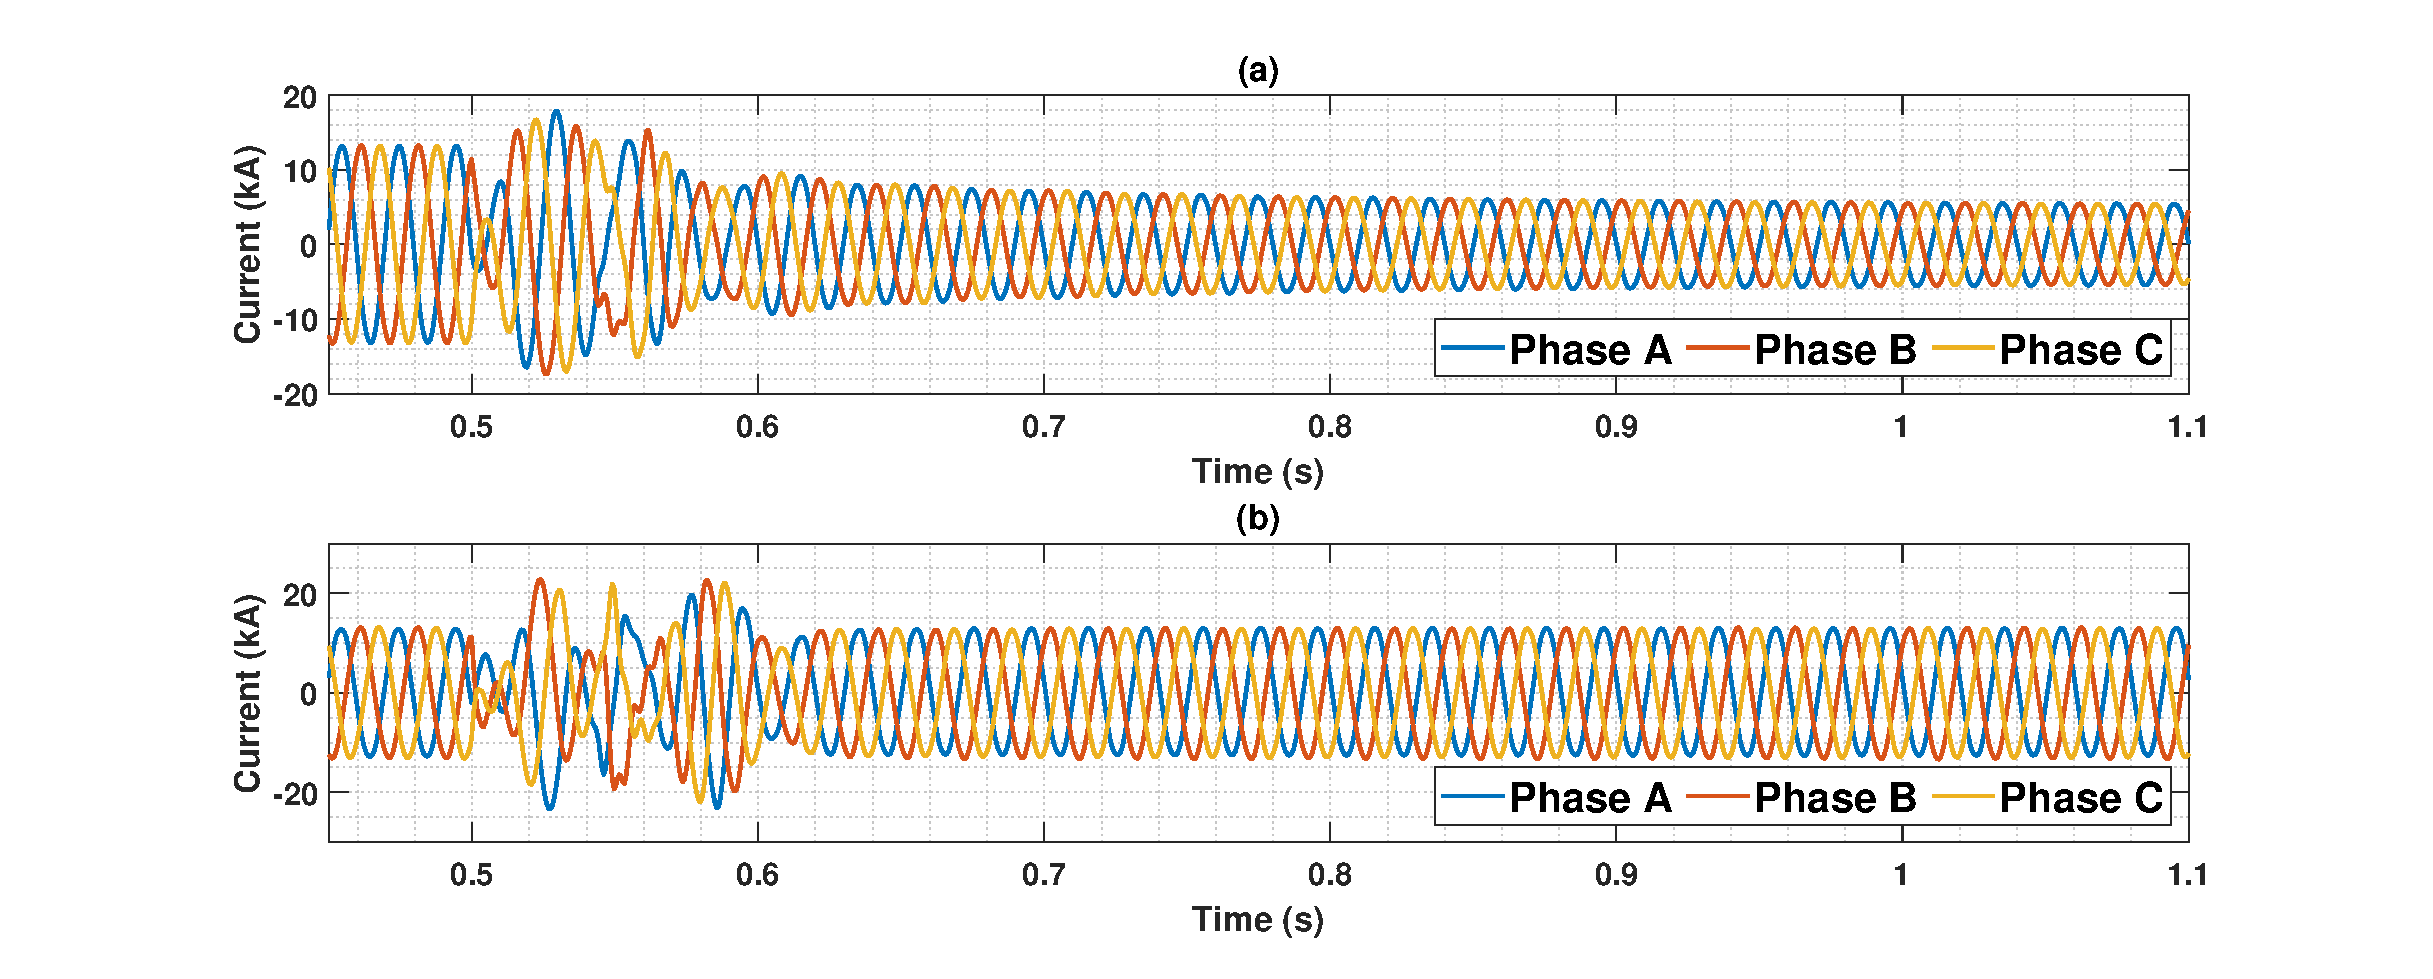
\includegraphics[height = 8.5cm,width = 18.5cm]{Diagrams/Chapter_5/IABC_MMC_1_2_3phaseSC.eps}
    \caption{Currents in a) MMC-1 connected bus and b) MMC-2 connected bus during three-phase line to ground fault in cable-1}
    \label{1516_3phaseSC}
\end{figure}

\begin{figure}[H]
\centering
%\hspace*{-1.2cm}
    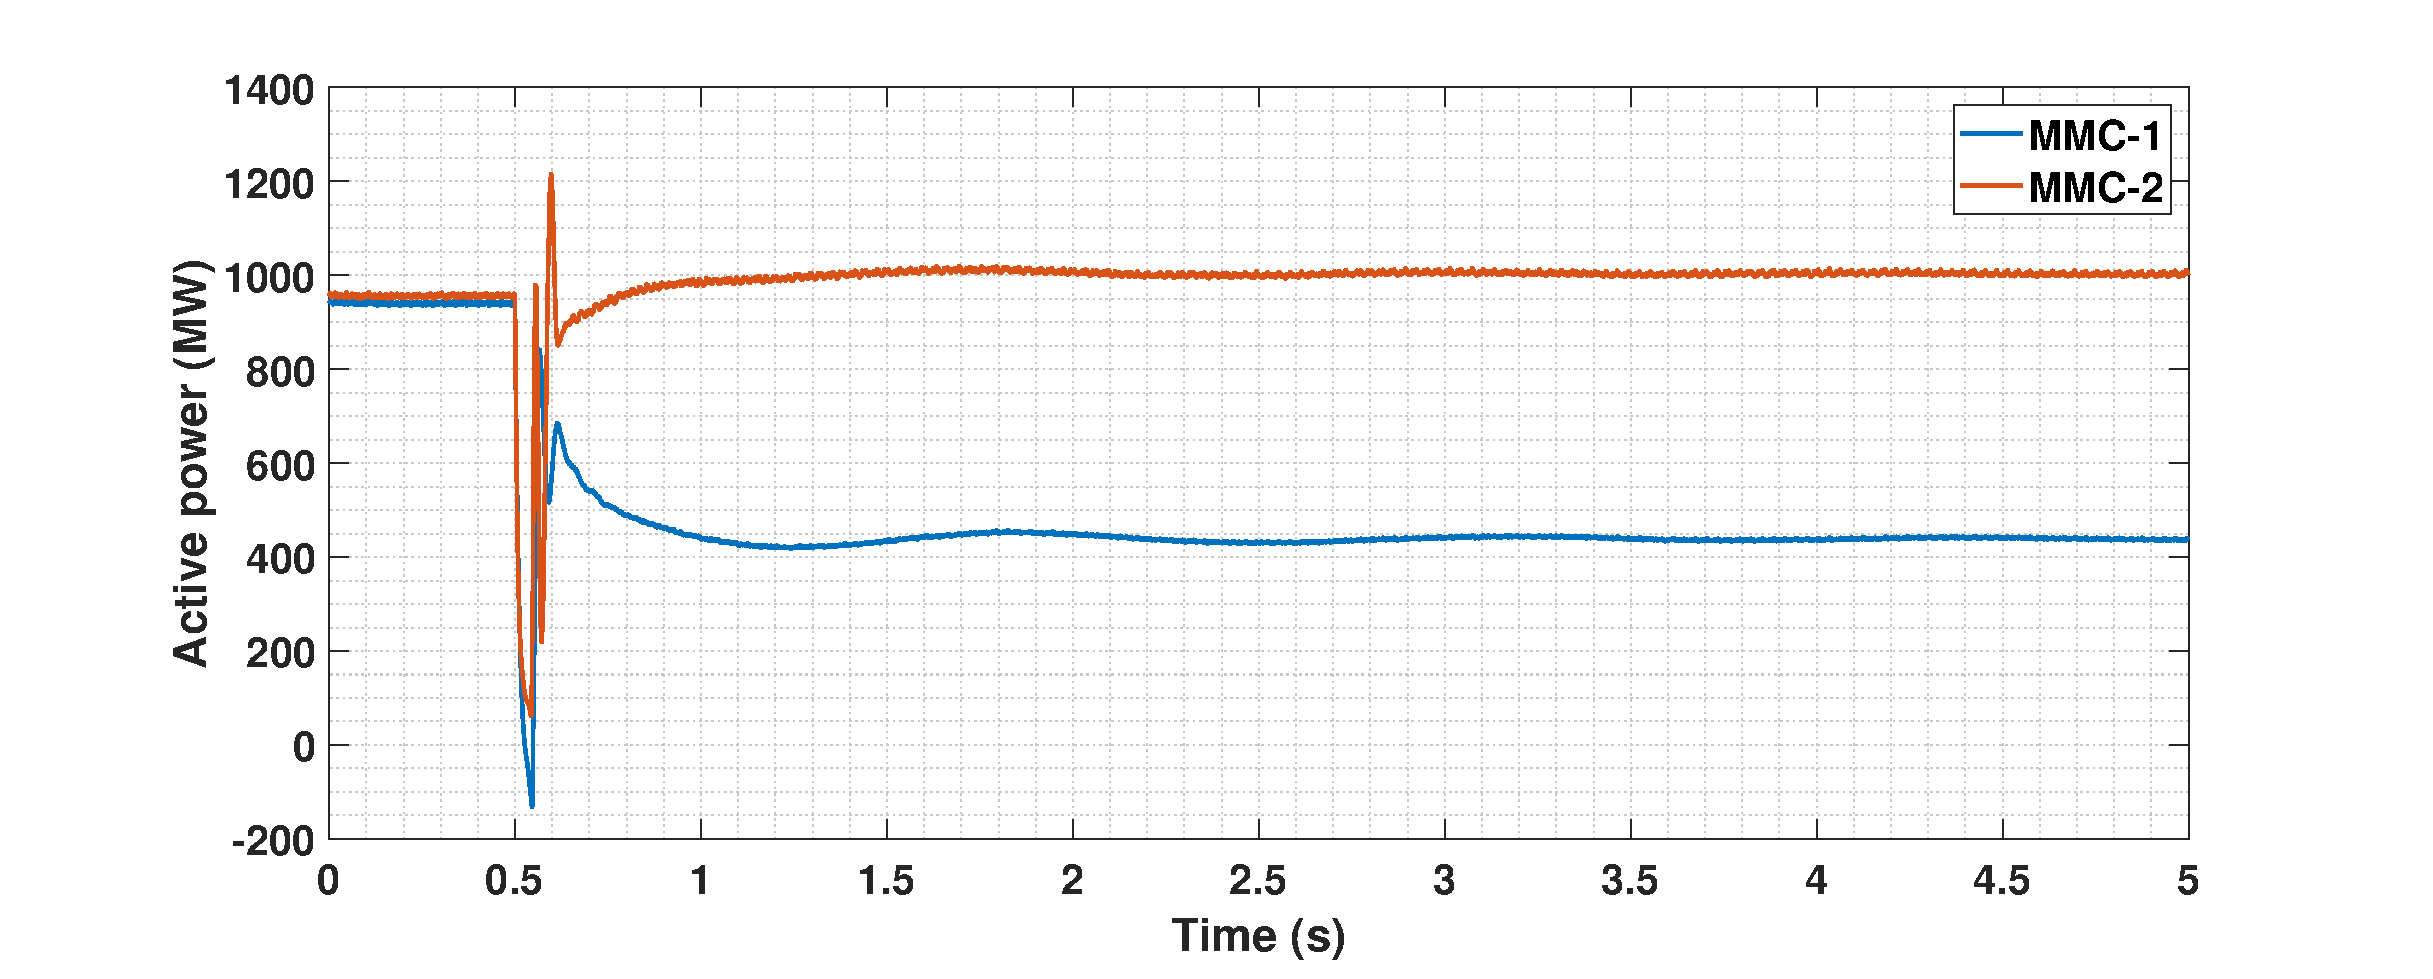
\includegraphics[height = 6.5cm,width = 9.25cm]{Diagrams/Chapter_5/P_MMC_1_2_3phaseSC.eps}
    \caption{Active power in MMC-1 bus and MMC-2 bus during three-phase line to ground fault in cable-1}
    \label{17_3phaseSC}
\end{figure}

Analysing at the \gls{WG} side of the network, the control is modelled to provide rated reactive current to flow to the fault location by controlling the voltage of the converter. From Figure \ref{WT1_voltages_3phasefault}, it can be seen that the voltage at the \gls{PCC}-1 drops and remains low throughout the fault period. During the time of fault, the angular reference of voltage at \gls{PCC}-1 is created by the \gls{PLL} modelled in the \gls{DVC} of \gls{WG}-1. This feature allows the implemented strategy to control the d-axis reference voltage of the \gls{GSC} and thereby indirectly controlling the current coming out of the \gls{GSC} to the \gls{PCC}. After the disconnection of \gls{WG}-1 from the network, the control allows reactive current thus reactive power to be passed through the fault location shown in Figure \ref{WT1_currents_3phasefault}. The current limitation algorithm implemented in the \gls{DVC} limits the current to the rating of the converter, hence rated reactive current flows from the \gls{GSC}.   
\begin{figure}[H]
\centering
%\hspace*{-1.2cm}
    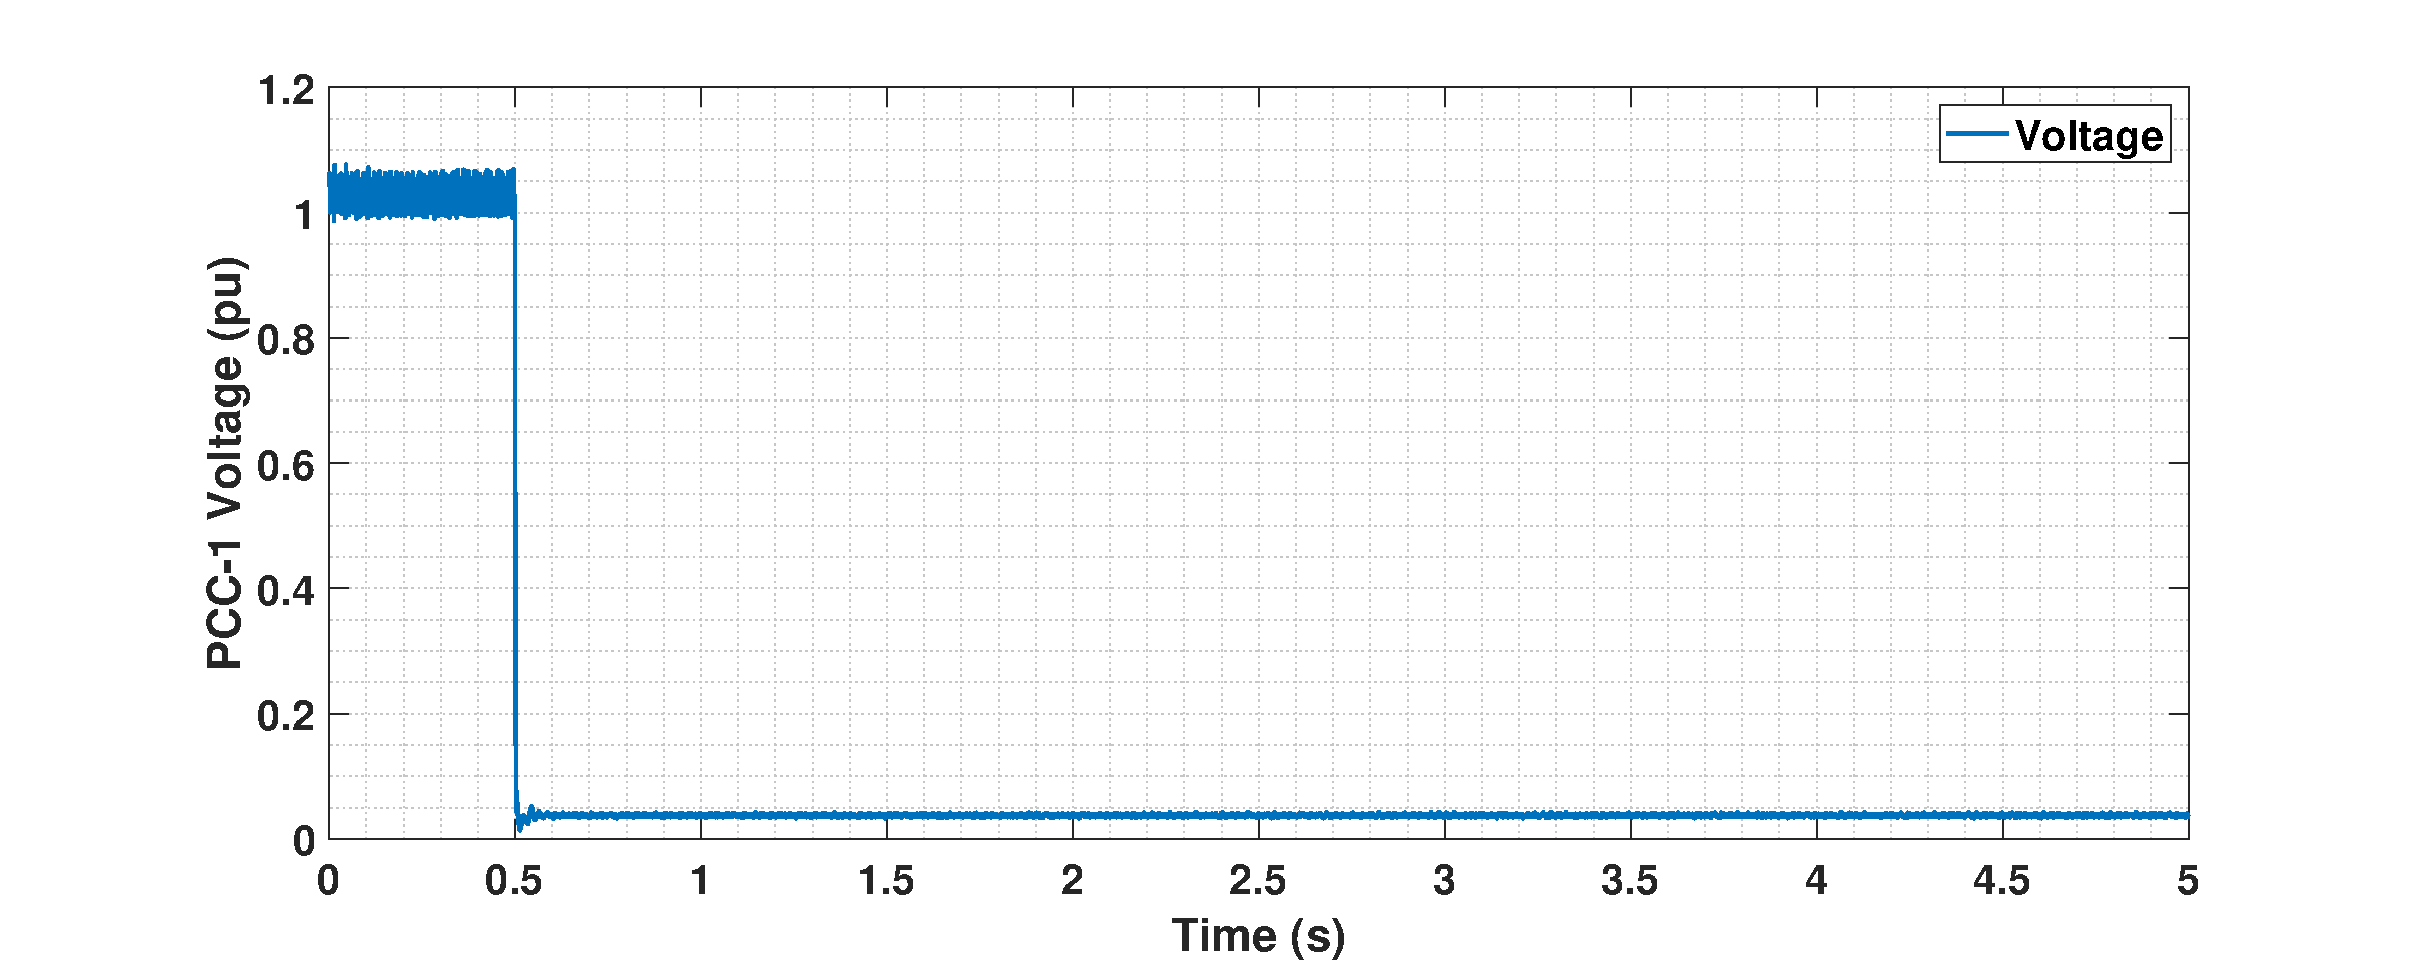
\includegraphics[height = 6.5cm,width = 9.25cm]{Diagrams/Chapter_5/VACP_WT1_3phaseSC.eps}
    \caption{Voltages at PCC-1 during three-phase line to ground fault in cable-1}
    \label{WT1_voltages_3phasefault}
\end{figure}

Also the voltages at the \gls{PCC} of \gls{WG}s- 2,3 and 4 have transients during the time of fault and is then stabilised to nearly a higher value than the pre-fault state. The post voltage value is within the tolerance limit ($\pm$10 \% ) and this can be viewed from the graphs in Figure \ref{VACP_WT234_3phaseSC} a). An important observation in the voltage graphs of \gls{WG}s -2,3 and 4 is the occurrence spikes right after the fault is released, as can be seen in Figure \ref{VACP_WT234_3phaseSC} b). The interactions between the \gls{PLL}s in the \gls{DVC}s and the \gls{PLL} in the U/F control as to which control dominates right when the fault is released, to calculate the angular reference can be understood to be the reason for this surge. This is an important issue faced by the industry experts are requires intensive research.

\begin{figure}[H]
\centering
%\hspace*{-1.2cm}
    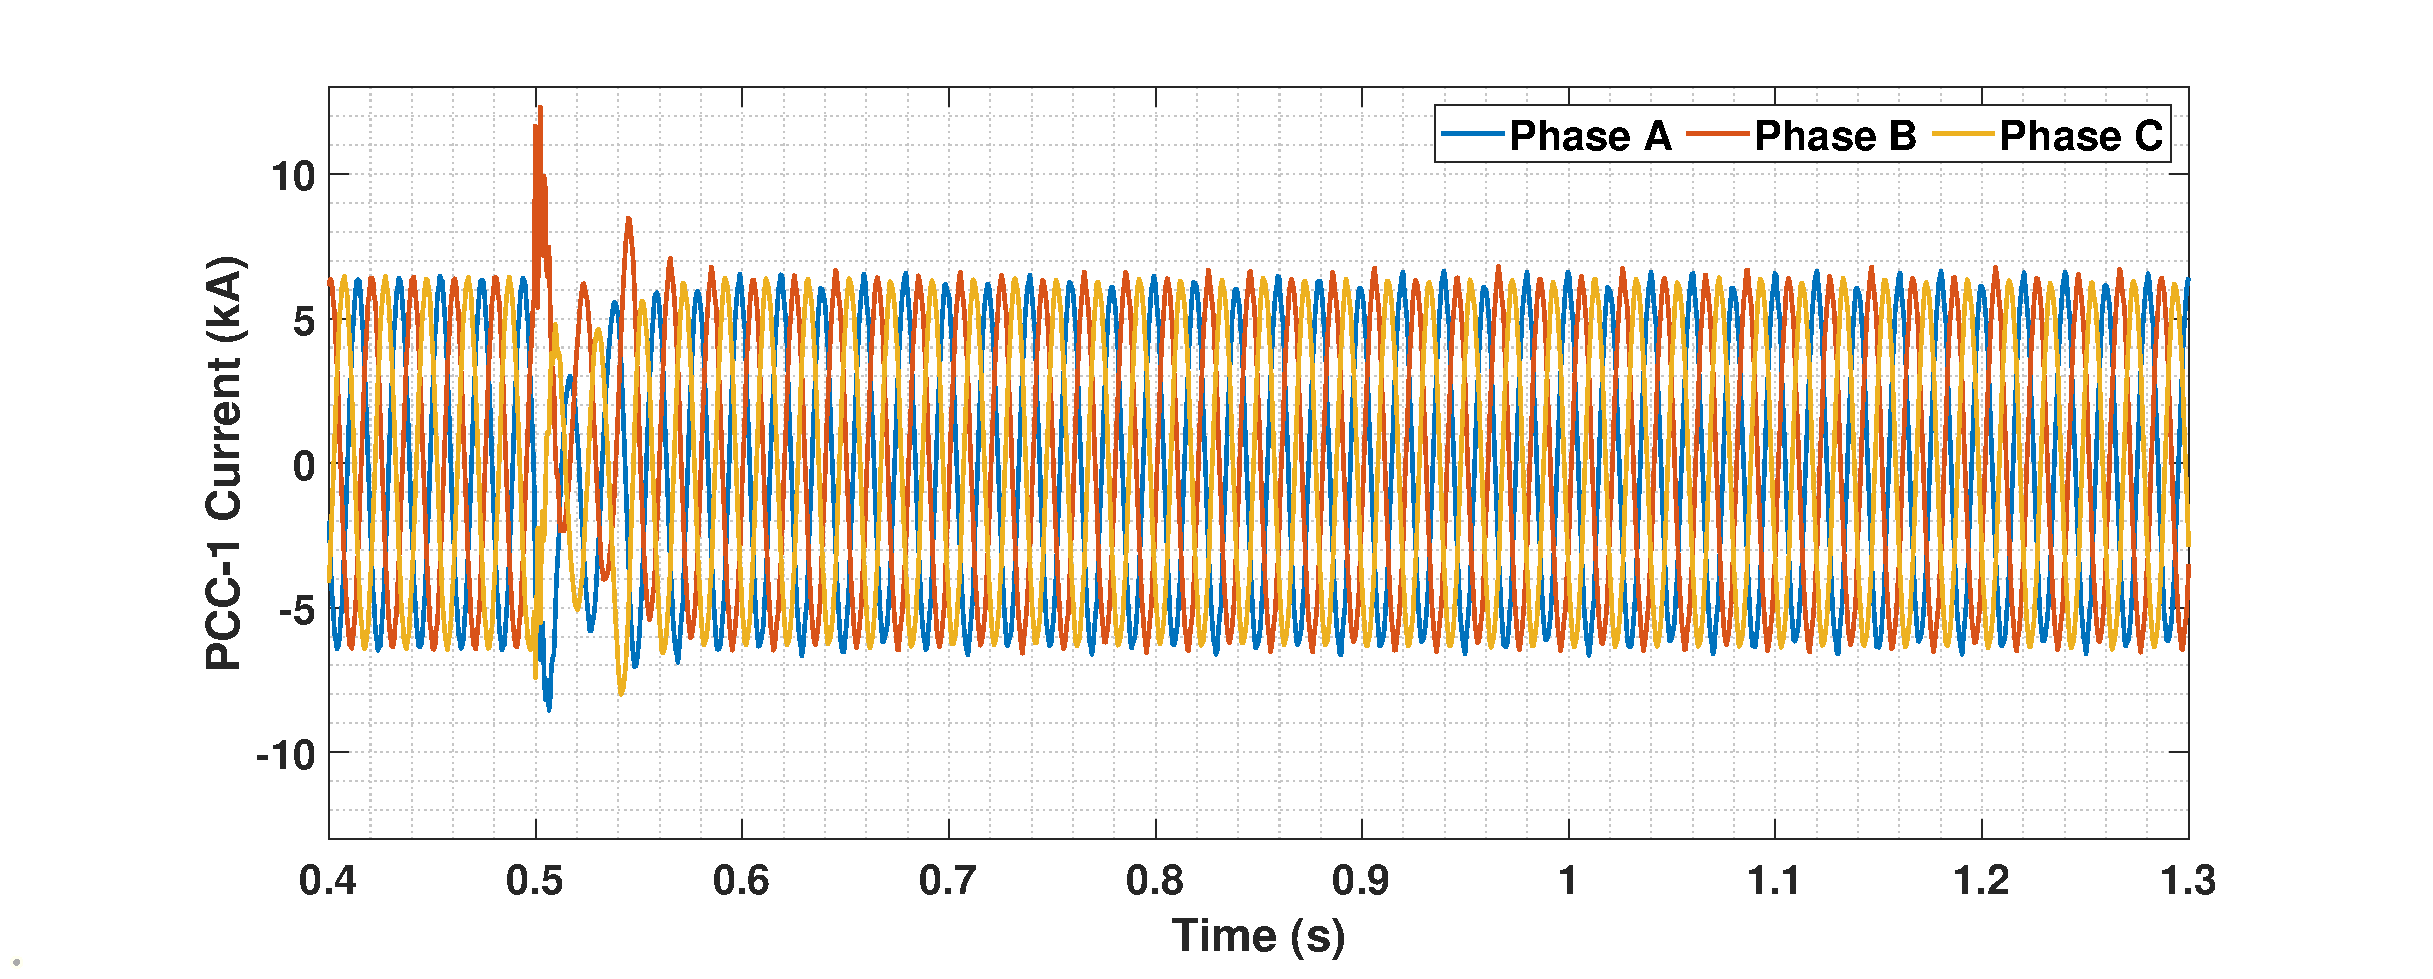
\includegraphics[height = 6.5cm,width = 17.25cm]{Diagrams/Chapter_5/IABC_WT1_3phaseSC.eps}
    \caption{Currents at PCC-1 during three-phase line to ground fault in cable-1}
    \label{WT1_currents_3phasefault}
\end{figure}


The currents from these other \gls{WG}s are slightly reduced in the post fault region (Figure \ref{IABC_WT234_3phaseSC}). The \gls{DVC} control in these \gls{WG}s operate during the time of fault and limit the currents by controlling the voltages at their respective \gls{PCC}s. These \gls{WG}s provide slightly higher amount of power as compared to the pre-fault state to be fed to the \gls{MMC}s due to the fact that the active power reference for \gls{MMC}-2 is set back to the initial value during the post fault period. Another important finding is in the profile of transients of currents during the occurrence of fault in \gls{WG}s-2,3 and 4. The current is limited during the time of fault and after the breaker has been operated, the profile is similar to that of the \gls{MMC}-2. This shows that \gls{MMC}-1 is dominating during the steady-state conditions and \gls{DVC} takes over control during dynamic scenarios. In practicality, since the fault occurs in the middle of the sea and it is difficult that the fault clears on its own, this control proves to be a valid strategy to control the voltage instabilities during the islanding of the offshore \gls{OWF}s. 

\begin{figure}[H]
%\centering
\hspace*{-1.2cm}
\captionsetup{justification=centering}
    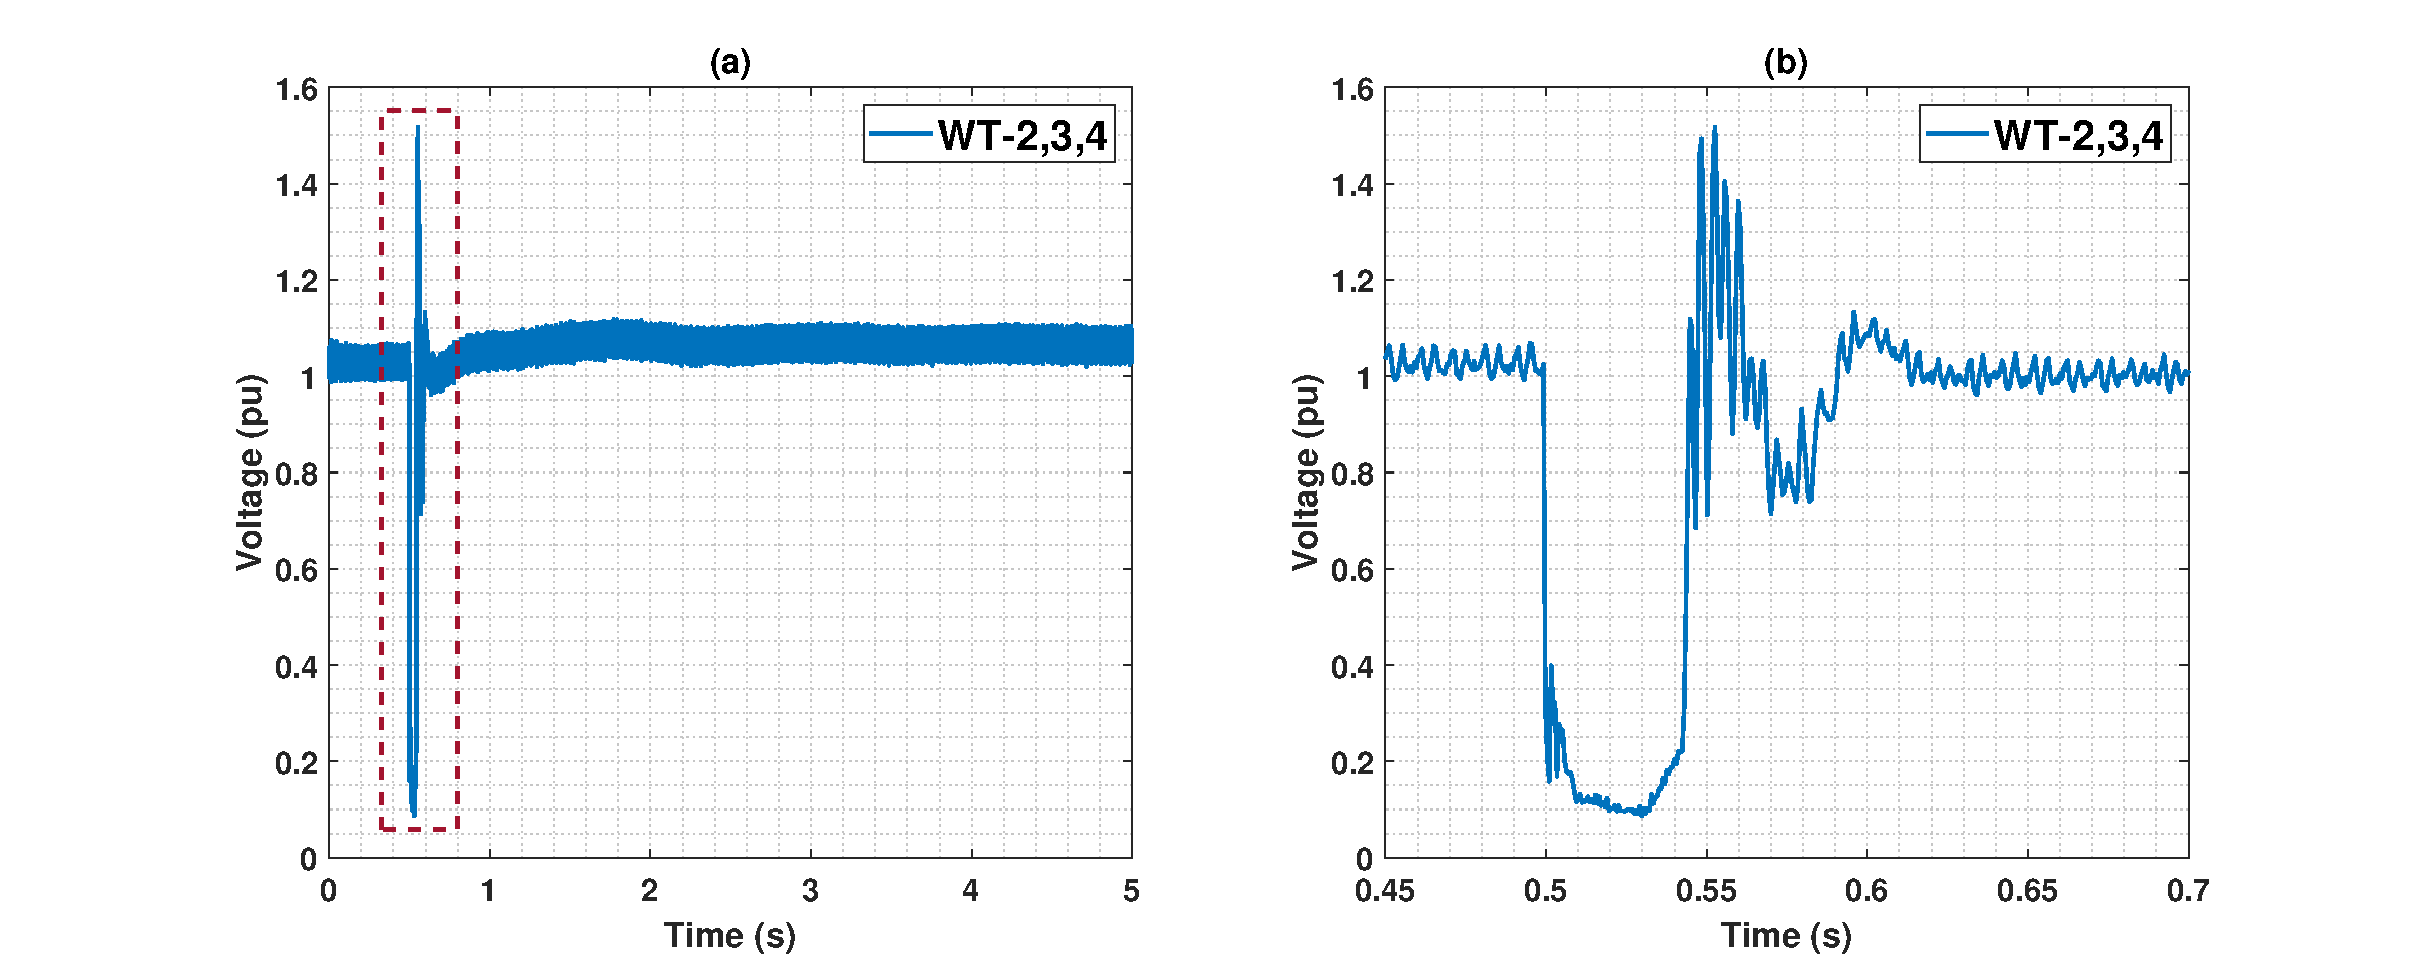
\includegraphics[height = 7.5cm,width = 19.25cm]{Diagrams/Chapter_5/VACP_WT234_3phaseSC.eps}
    \caption{a) Voltages at PCC-2, 3 and 4 during three phase short circuit in cable-1 b) Zoom-in of voltages at PCC-2, 3 and 4 during three phase short circuit in cable-1}
    \label{VACP_WT234_3phaseSC}
\end{figure}
%\vspace{-2mm}


\begin{figure}[H]
\centering
%\hspace*{-1.2cm}
\captionsetup{justification=centering}
    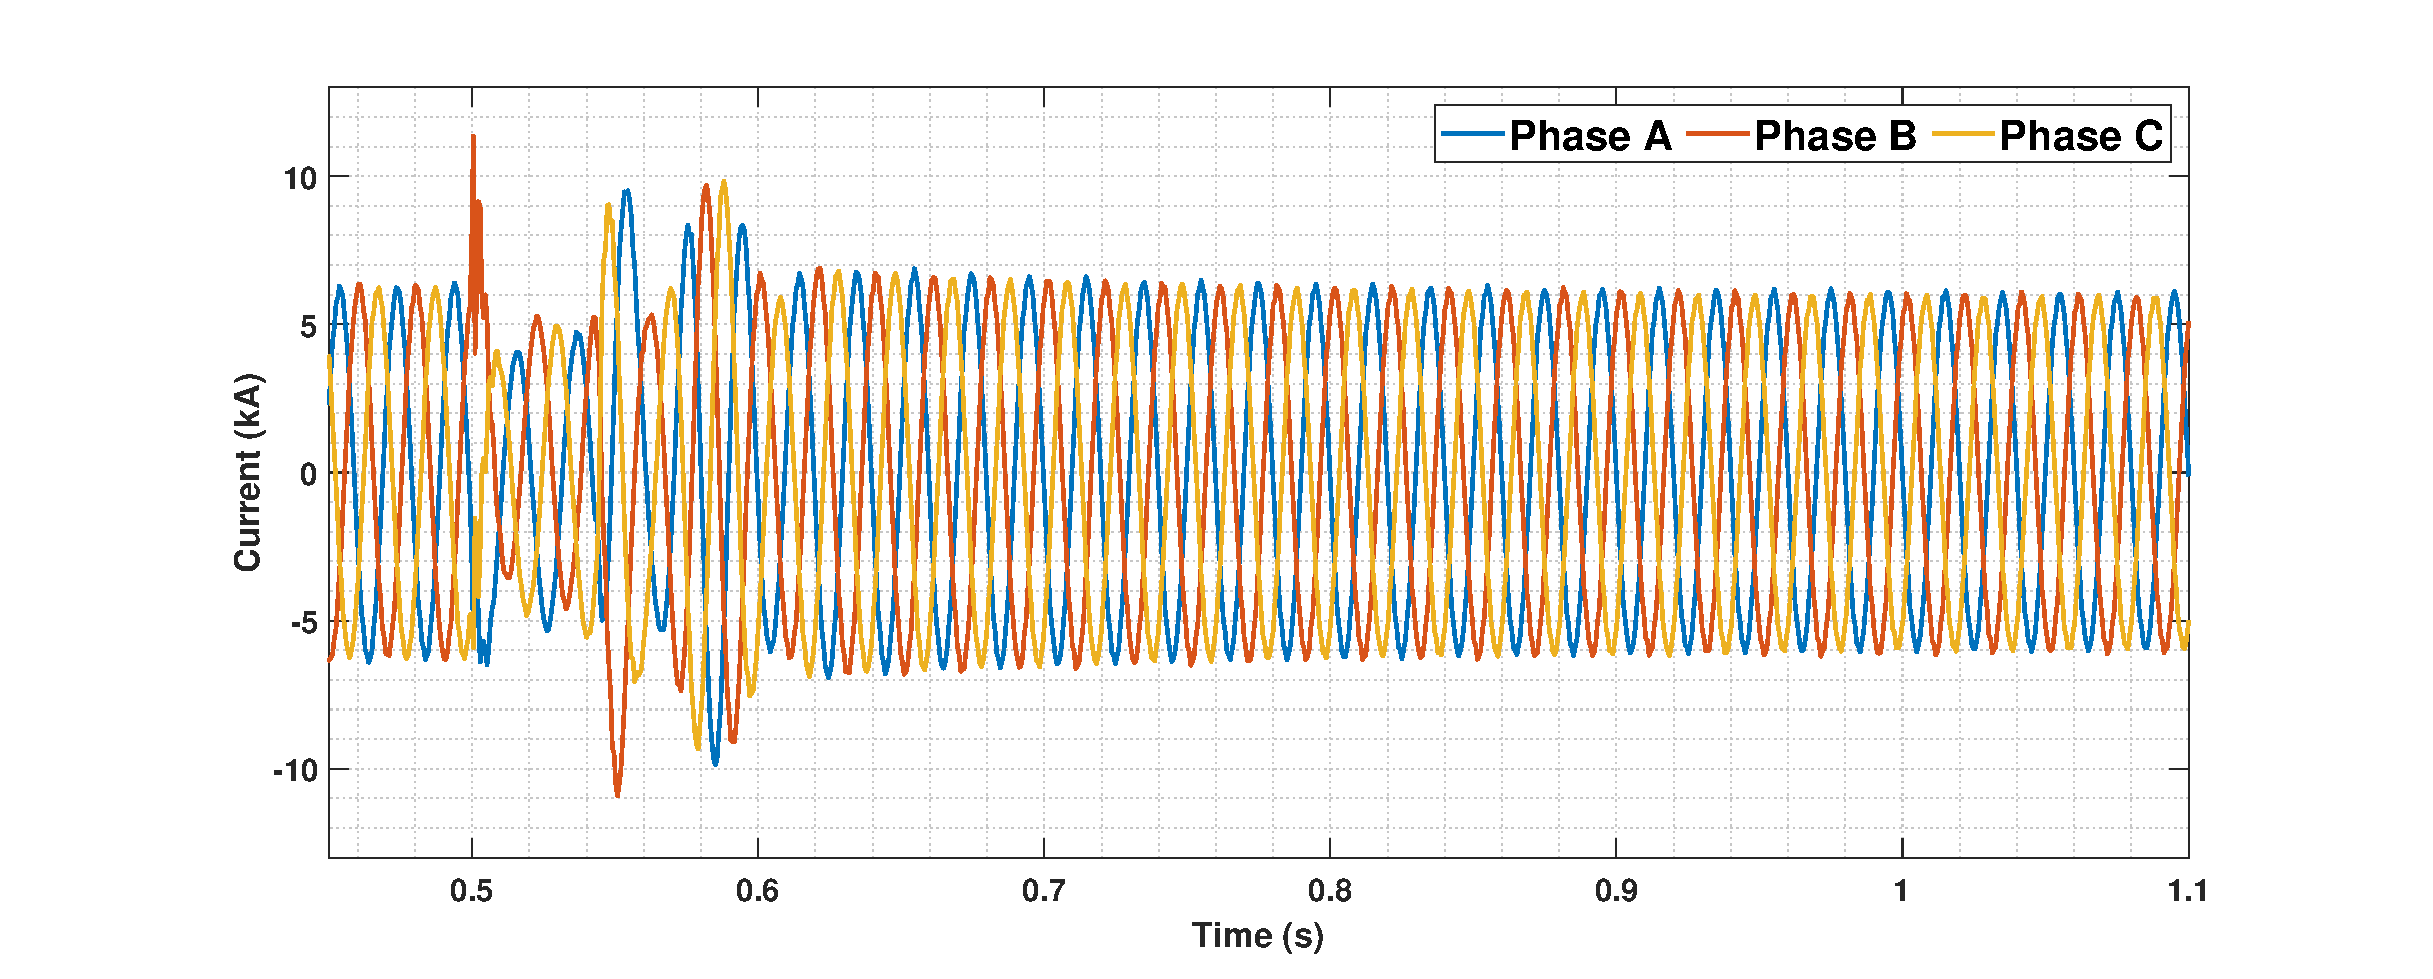
\includegraphics[height = 6.5cm,width = 17.25cm]{Diagrams/Chapter_5/IABC_WT234_3phaseSC.eps}
    \caption{Currents at PCC-2, 3 and 4 during three-phase line to ground fault in cable-1}
    \label{IABC_WT234_3phaseSC}
\end{figure}

As per the available grid codes mentioned in \cite{mohseni_review_2012}, during normal operation active current must be the priority and during the time of fault the priority must be changed to reactive current. The major takeaway from this chapter is that, the \gls{DVC} follows the reactive current injection requirement during the time of fault as shown in Figure \ref{18_3phaseSC} a) even while working in coordination with other controls in the network. The current is limited to the rated current of the converter by the current limitation algorithm in \gls{DVC} without requirement of any external controls. Simultaneously, the currents in the other \gls{WG}s are balanced as per the active power required in \gls{MMC}-2 as seen in Figure \ref{18_3phaseSC} b). 
\vspace{-3mm}
\begin{figure}[H]
%\centering
\hspace*{-1.2cm}
    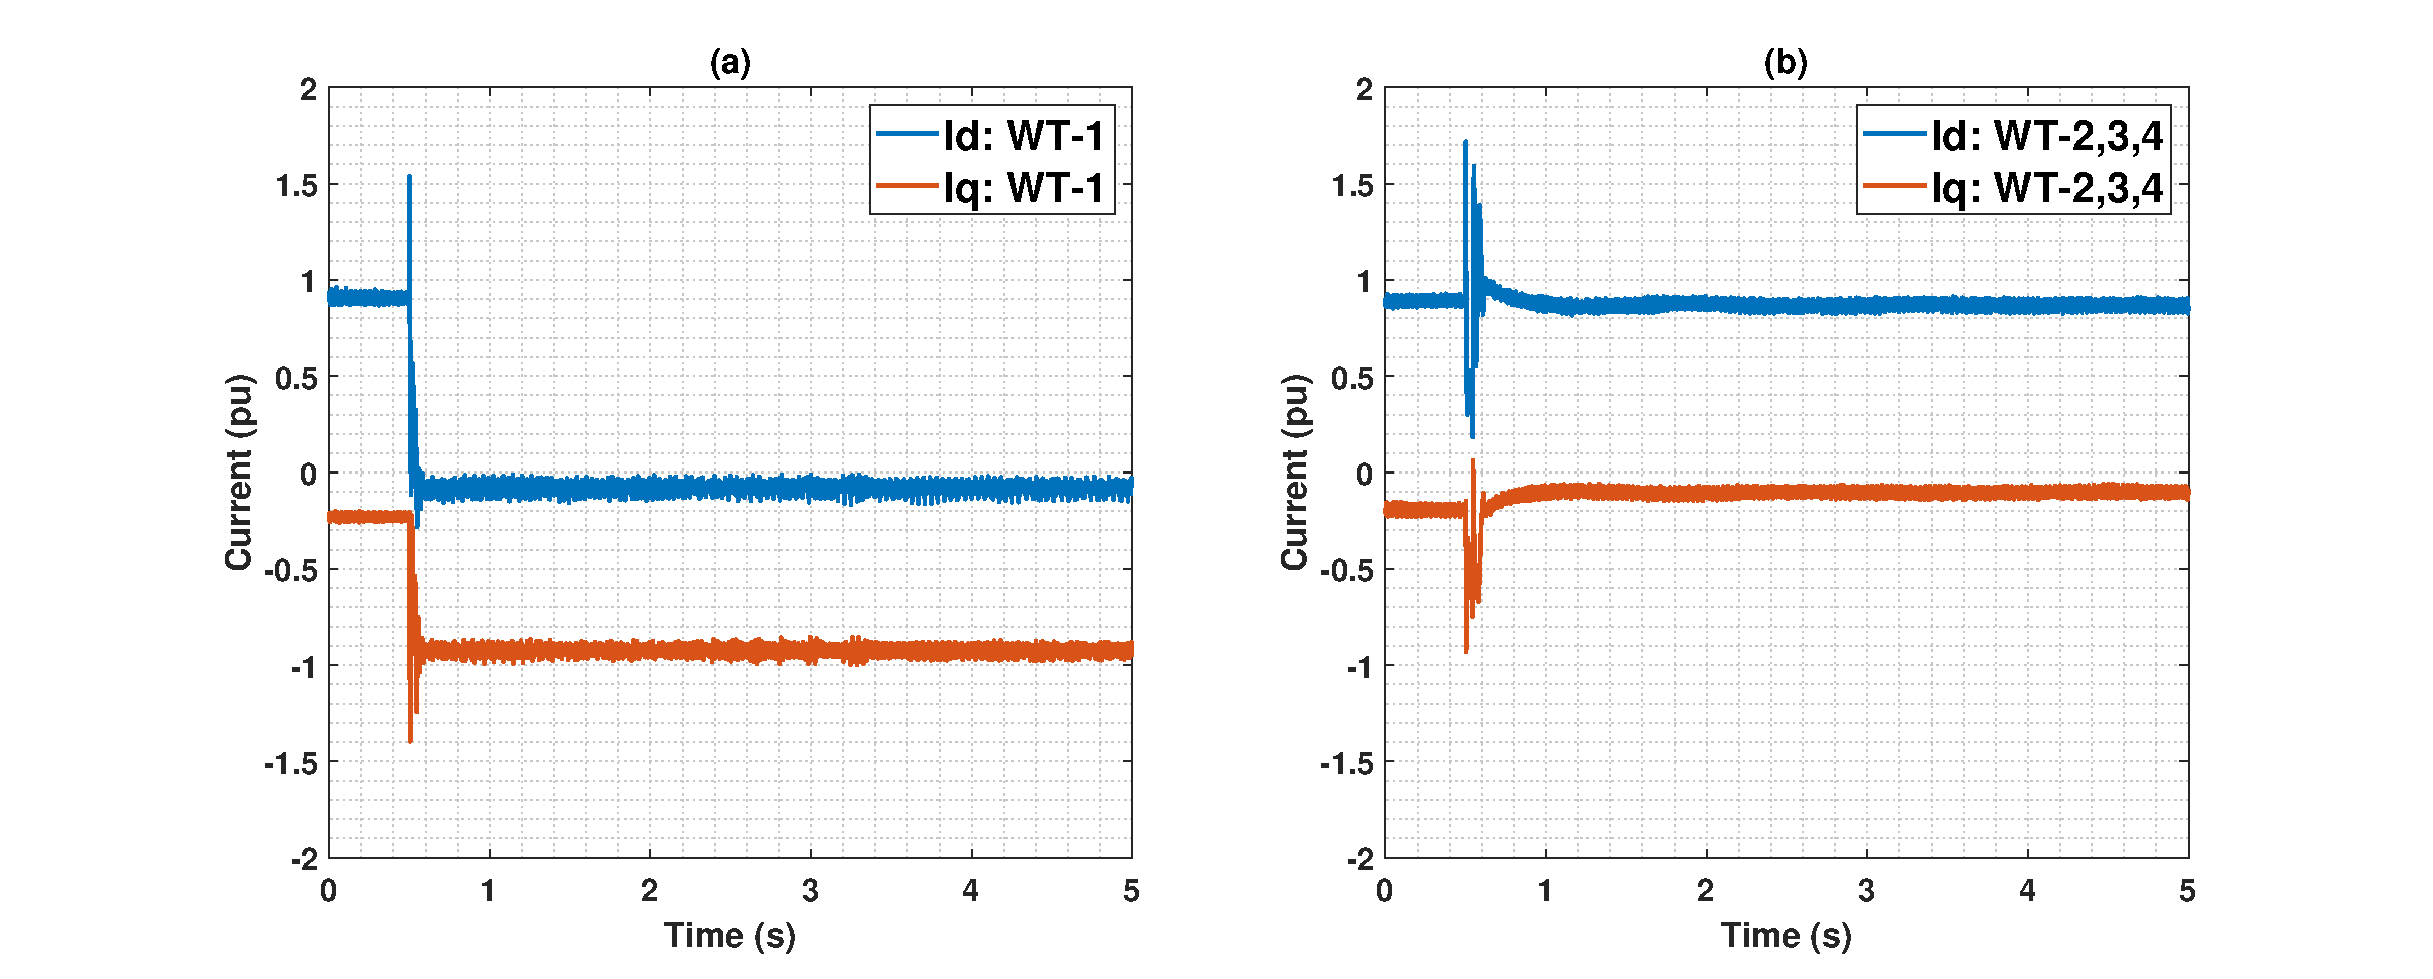
\includegraphics[height = 6cm,width = 17.25cm]{Diagrams/Chapter_5/IDQ_WT1234_3phaseSC.eps}
    \caption{Currents in d and q axes at PCC-1 during three-phase line to ground fault in cable-1}
    \label{18_3phaseSC}
\end{figure}
